% report/ExpEmain000.tex
\documentclass[18pt,c]{beamer}
\makeatletter
\let\beamer@writeslidentry@miniframeson=\beamer@writeslidentry
\def\beamer@writeslidentry@miniframesoff{%
  \expandafter\beamer@ifempty\expandafter{\beamer@framestartpage}{}% does not happen normally
  {%else
    % removed \addtocontents commands
   \clearpage\beamer@notesactions%
  }
}
\newcommand*{\miniframeson}{\let\beamer@writeslidentry=\beamer@writeslidentry@miniframeson}
\newcommand*{\miniframesoff}{\let\beamer@writeslidentry=\beamer@writeslidentry@miniframesoff}
\makeatother
% yellow
\definecolor{goldenyellow}{rgb}{1.0, 0.87, 0.0}
\definecolor{electricyellow}{rgb}{1.0, 1.0, 0.0}
\definecolor{icterine}{rgb}{0.99, 0.97, 0.37}
\definecolor{flavescent}{rgb}{0.97, 0.91, 0.56}
\definecolor{lemon}{rgb}{1.0, 0.97, 0.0}
% orange
\definecolor{amber}{rgb}{1.0, 0.75, 0.0}
\definecolor{cadmiumorange}{rgb}{0.93, 0.53, 0.18}
\definecolor{internationalorange}{rgb}{1.0, 0.31, 0.0}
% red
\definecolor{ferrarired}{rgb}{1.0, 0.11, 0.0}
\definecolor{fireenginered}{rgb}{0.81, 0.09, 0.13}
\definecolor{cadmiumred}{rgb}{0.89, 0.0, 0.13}
% blue
\definecolor{ao}{rgb}{0.0, 0.5, 0.0}
\definecolor{babyblueeyes}{rgb}{0.63, 0.79, 0.95}
\definecolor{bleudefrance}{rgb}{0.19, 0.55, 0.91}
\definecolor{blue}{rgb}{0.0, 0.0, 1.0}
\definecolor{cobalt}{rgb}{0.0, 0.28, 0.67}
\definecolor{darkmidnightblue}{rgb}{0.0, 0.2, 0.4}
\definecolor{brandeisblue}{rgb}{0.0, 0.44, 1.0}
\definecolor{deepskyblue}{rgb}{0.0, 0.75, 1.0}
\definecolor{iris}{rgb}{0.35, 0.31, 0.81}
\definecolor{navyblue}{rgb}{0.0, 0.0, 0.5}
\definecolor{ultramarine}{rgb}{0.07, 0.04, 0.56}
\definecolor{electricultramarine}{rgb}{0.25, 0.0, 1.0}
% green
\definecolor{cadmiumgreen}{rgb}{0.0, 0.42, 0.24}
\definecolor{darkpastelgreen}{rgb}{0.01, 0.75, 0.24}
\usetheme{Berlin}
\usecolortheme{default}
\usefonttheme{default}
\setbeamercolor{structure}{fg=ferrarired}
\setbeamerfont{frametitle}{size=\footnotesize}
\usepackage{graphicx}
\renewcommand{\topfraction}{1.0}
\renewcommand{\floatpagefraction}{1.0}
\begin{document}
\title{Report of Experiment ExpE. k-Symmetry: Grammar Tuning and Language Tuning}
\author{Andreas Geyer-Schulz}
\date{\today}
\begin{frame}
\titlepage
\end{frame}
\begin{frame}
\frametitle{Abstract}
Grammar tuning adapts the language. Language tuning adds new language elements. In this experiment we compare the best grammar of experiment B with a grammar with symmetric pairs and an additional function.%\end{abstract}
\end{frame}
\begin{frame}[t, allowframebreaks]
\frametitle{Contents}
\tableofcontents[subsubsectionstyle=hide]
\vfill
\end{frame}
% report/ExpEmain001.tex
\miniframeson
\section{Design of Experiment}
% report/ExpEmain002.tex
\begin{frame}
\vspace*{2mm}
\begin{block}{
Definition
}
{\bf Grammar tuning} means adding additional production rules
to a context-free grammar with the goal of improving the learning
performance of grammar-based genetic programming algorithms.
 
{\bf Example:} Repeating production rules allows to change the distribution
of programs (and their sizes) generated during the initialization a grammar-based
genetic programming algorithm.
\end{block}
\end{frame}% report/ExpEmain003.tex
\begin{frame}
\vspace*{2mm}
\begin{block}{
Definition
}
{\bf Language tuning} means adding additional language elements.
This means changing the grammar {\bf and} the syntax of the language elements
and changing the implementation of the language so that the semantics
of the language is implemented.
 
{\bf Example:} Adding a new base function. E.g. NAND.
\end{block}
\end{frame}% report/ExpEmain004.tex
\begin{frame}
\vspace*{2mm}
\begin{block}{
Description of Experiment
}
The purpose of this computational experiment is to show the improvement
of performance by grammar {\bf and} language tuning.
 
The {\bf problem environment} is the k-symmetry problem: 
Finding a boolean expression (with and, or, and not)
which is TRUE for symmetric k-bit strings.
 
The {\bf solution method} is grammar-based genetic programming
(option {\tt algorithm="sgp"}  of {\tt xegaRun}).
The {\bf solver} used is {\tt xegaRun} from the R-package {\tt xega}.
 
The experiment consists of 10 treatments, 2 grammars for 5 problem sizes $k\in 2,\dots, 6$.
\end{block}
\end{frame}% report/ExpEmain005.tex
\begin{frame}
\frametitle{
Description of Experiment
}
The two control variables in this experiment are
\begin{itemize}
\item The bit-length of the k-symmetry problem: 2, 3, 4, 5, and 6.
\item The grammar for boolean expressions:
\begin{itemize} 
\item {\bf T4}: With two rules for OR and two rules for variables replaced
            by symmetric pairs.
\item {\bf T5}: With symmetric pairs and a new base function,
       the function sPair(x, y) which implements
 
sPair $<-$ function)x,y) {OR(AND(x,y),AND(NOT(x),NOT(y)))}
\end{itemize}
\end{itemize}
\end{frame}% report/ExpEmain006.tex
% ExpE
% Table: Common Parameters of Experiment ExpE
% Thu May  8 17:40:53 2025
 \begin{frame}
 \fontsize{8pt}{9pt}\selectfont
 \frametitle{ Common Parameters of Experiment ExpE }
% latex table generated in R 4.4.3 by xtable 1.8-4 package
% Wed May 14 17:33:39 2025
\begin{table}[ht]
\centering
\begin{tabular}{rr}
  \hline
 & Parameter Value \\ 
  \hline
Optimize & Minimize! \\ 
  Trials & 80 \\ 
  Algorithm & sgp \\ 
  Max.Depth.of.DTs & 7 \\ 
  Replay & 0 \\ 
  Evaluation.Method & Deterministic \\ 
  Execution.Model & MultiCore \\ 
  Verbose & 1 \\ 
  Semantics & byValue \\ 
  Report.Eval.Errors & TRUE \\ 
  Termination.Condition & AbsoluteError \\ 
  Termination.Eps & -0.1 \\ 
  Gene.Map & Bin2Dec \\ 
  Init.Gene & InitGene \\ 
  Codon.Precision & LCM \\ 
   \hline
\end{tabular}
\caption{Common Parameters of Experiment ExpE (Part 1)} 
\end{table}

 \label{ExpECommonTable000.tex}  
 \end{frame}

 % Label:  \label{ExpECommonTable000.tex}  
% report/ExpEmain007.tex
% ExpE
% Table: Common Parameters of Experiment ExpE
% Thu May  8 17:40:53 2025
 \begin{frame}
 \fontsize{8pt}{9pt}\selectfont
 \frametitle{ Common Parameters of Experiment ExpE }
% latex table generated in R 4.4.3 by xtable 1.8-4 package
% Thu May  8 17:40:53 2025
\begin{table}[ht]
\centering
\begin{tabular}{rr}
  \hline
 & Parameter Value \\ 
  \hline
Population.Size & 200 \\ 
  Max.Generations & 500 \\ 
  Crossover.Rate & 0.2 \\ 
  Mutation.Rate & 0.4 \\ 
  IV.Crossover.Rate & Const \\ 
  Crossover.Rate.2 & 0.4 \\ 
  IV.Mutation.Rate & Const \\ 
  Mutation.Rate.2 & 0.8 \\ 
   \hline
\end{tabular}
\caption{Common Parameters of Experiment ExpE (Part 2)} 
\end{table}

 \label{ExpECommonTable001.tex}  
 \end{frame}

 % Label:  \label{ExpECommonTable001.tex}  
% report/ExpEmain008.tex
% ExpE
% Table: Parameters of Treatments of Experiment ExpE
% Thu May  8 17:40:53 2025
 \begin{frame}
 \fontsize{8pt}{9pt}\selectfont
 \frametitle{ Parameters of Treatments of Experiment ExpE }
% latex table generated in R 4.4.3 by xtable 1.8-4 package
% Thu May  8 17:40:53 2025
\begin{table}[ht]
\centering
\begin{tabular}{rrrrrrr}
  \hline
 & Experiment & Treatment & Problem Environment & Grammar & Worst Fitness & Codons \\ 
  \hline
1 & EB & BoolT4sgp2k & 2-Symmetry Problem & AndOrNotTuned4.txt &  -4 &  80 \\ 
  2 & EB & BoolT4sgp3k & 3-Symmetry Problem & AndOrNotTuned4.txt &  -8 & 120 \\ 
  3 & EB & BoolT4sgp4k & 4-Symmetry Problem & AndOrNotTuned4.txt & -16 & 160 \\ 
  4 & EB & BoolT4sgp5k & 5-Symmetry Problem & AndOrNotTuned4.txt & -32 & 200 \\ 
  5 & EB & BoolT4sgp6k & 6-Symmetry Problem & AndOrNotTuned4.txt & -64 & 240 \\ 
  6 & EE & BoolT5sgp2k & 2-Symmetry Problem & AndOrNotTuned5.txt &  -4 &  80 \\ 
  7 & EE & BoolT5sgp3k & 3-Symmetry Problem & AndOrNotTuned5.txt &  -8 & 120 \\ 
  8 & EE & BoolT5sgp4k & 4-Symmetry Problem & AndOrNotTuned5.txt & -16 & 160 \\ 
  9 & EE & BoolT5sgp5k & 5-Symmetry Problem & AndOrNotTuned5.txt & -32 & 200 \\ 
  10 & EE & BoolT5sgp6k & 6-Symmetry Problem & AndOrNotTuned5.txt & -64 & 240 \\ 
   \hline
\end{tabular}
\caption{Parameters of Treatments of Experiment ExpE} 
\end{table}

 \label{ExpEDifferentTable000.tex}  
 \end{frame}

 % Label:  \label{ExpEDifferentTable000.tex}  
% report/ExpEmain009.tex
\miniframeson
\section{Exploratory Analysis}
% report/ExpEmain010.tex
\miniframeson
\subsection{Do we always find an optimal solution?}
% report/ExpEmain011.tex
% ExpE
% Table: Matrix of Mean of Errors (Fitness).  Rows: k=2, 3, 4, 5, 6)
% Thu May  8 17:40:53 2025
 \begin{frame}
 \fontsize{8pt}{9pt}\selectfont
 \frametitle{ Matrix of Mean of Errors (Fitness).  Rows: k=2, 3, 4, 5, 6) }
% latex table generated in R 4.4.3 by xtable 1.8-4 package
% Wed May 14 17:33:40 2025
\begin{table}[ht]
\centering
\begin{tabular}{rrr}
  \hline
 & T4 & T5 \\ 
  \hline
1 & 0.00 & 0.00 \\ 
  2 & 0.00 & 0.00 \\ 
  3 & 0.00 & 0.00 \\ 
  4 & 0.00 & 0.00 \\ 
  5 & 3.33 & 0.00 \\ 
   \hline
\end{tabular}
\caption{Matrix of Mean of Errors (Fitness).  Rows: k=2, 3, 4, 5, 6)} 
\end{table}

 \label{ExpEMeanMatrixTable000.tex}  
 \end{frame}

 % Label:  \label{ExpEMeanMatrixTable000.tex}  
% report/ExpEmain012.tex
% ExpE
% Table: Matrix of Min of Errors (Fitness). Rows: k=2, 3, 4, 5, 6)
% Thu May  8 17:40:54 2025
 \begin{frame}
 \fontsize{8pt}{9pt}\selectfont
 \frametitle{ Matrix of Min of Errors (Fitness). Rows: k=2, 3, 4, 5, 6) }
% latex table generated in R 4.4.3 by xtable 1.8-4 package
% Wed May 14 17:33:40 2025
\begin{table}[ht]
\centering
\begin{tabular}{rrr}
  \hline
 & T4 & T5 \\ 
  \hline
1 & 0.00 & 0.00 \\ 
  2 & 0.00 & 0.00 \\ 
  3 & 0.00 & 0.00 \\ 
  4 & 0.00 & 0.00 \\ 
  5 & 0.00 & 0.00 \\ 
   \hline
\end{tabular}
\caption{Matrix of Min of Errors (Fitness). Rows: k=2, 3, 4, 5, 6)} 
\end{table}

 \label{ExpEMeanMatrixTable001.tex}  
 \end{frame}

 % Label:  \label{ExpEMeanMatrixTable001.tex}  
% report/ExpEmain013.tex
\begin{frame}
\frametitle{
Do we always find the optimal program?
}
\begin{itemize}
\item For grammar T5: {\bf Yes.}
       For grammar T4: {\bf No.}
       (Not for the 6-symmetry problem with 500 generations.
\item For the 6-symmetry problem, the grammar T4 has maximum of 6 errors.
\end{itemize}
\end{frame}% report/ExpEmain014.tex
\miniframeson
\subsection{How long to find an optimal solution?}
% report/ExpEmain015.tex
% ExpE
% Table: Matrix of Mean of Seconds.  Rows: k=2, 3, 4, 5, 6)
% Thu May  8 17:40:54 2025
 \begin{frame}
 \fontsize{8pt}{9pt}\selectfont
 \frametitle{ Matrix of Mean of Seconds.  Rows: k=2, 3, 4, 5, 6) }
% latex table generated in R 4.4.3 by xtable 1.8-4 package
% Wed May 14 17:33:40 2025
\begin{table}[ht]
\centering
\begin{tabular}{rrr}
  \hline
 & T4 & T5 \\ 
  \hline
1 & 0.24 & 0.22 \\ 
  2 & 0.30 & 0.25 \\ 
  3 & 17.93 & 0.31 \\ 
  4 & 18.16 & 0.34 \\ 
  5 & 193.42 & 1.93 \\ 
   \hline
\end{tabular}
\caption{Matrix of Mean of Seconds.  Rows: k=2, 3, 4, 5, 6)} 
\end{table}

 \label{ExpEMeanMatrixTable002.tex}  
 \end{frame}

 % Label:  \label{ExpEMeanMatrixTable002.tex}  
% report/ExpEmain016.tex
% ExpE
% Table: Matrix of Mean of Generations.  Rows: k=2, 3, 4, 5, 6)
% Thu May  8 17:40:54 2025
 \begin{frame}
 \fontsize{8pt}{9pt}\selectfont
 \frametitle{ Matrix of Mean of Generations.  Rows: k=2, 3, 4, 5, 6) }
% latex table generated in R 4.4.3 by xtable 1.8-4 package
% Wed May 14 17:33:40 2025
\begin{table}[ht]
\centering
\begin{tabular}{rrr}
  \hline
 & T4 & T5 \\ 
  \hline
1 & 1.00 & 1.00 \\ 
  2 & 1.01 & 1.00 \\ 
  3 & 77.01 & 1.23 \\ 
  4 & 73.10 & 1.20 \\ 
  5 & 460.68 & 7.22 \\ 
   \hline
\end{tabular}
\caption{Matrix of Mean of Generations.  Rows: k=2, 3, 4, 5, 6)} 
\end{table}

 \label{ExpEMeanMatrixTable003.tex}  
 \end{frame}

 % Label:  \label{ExpEMeanMatrixTable003.tex}  
% report/ExpEmain017.tex
% ExpE
% Figure: Distribution of Number of Generations for Grammars. 2k  symmetry.
% Thu May  8 17:40:54 2025
 \begin{frame}
 \frametitle{ Distribution of Number of Generations for Grammars. 2k  symmetry. }
 \begin{center}
\includegraphics[width=0.5\textwidth, angle=-90]
{ExpEboxplottGenerations000.eps}
 \end{center}
 \label{ExpEboxplottGenerations000.eps}  
 \end{frame}

% report/ExpEmain018.tex
% ExpE
% Figure: Distribution of Number of Generations for Grammars. 3k  symmetry.
% Thu May  8 17:40:54 2025
 \begin{frame}
 \frametitle{ Distribution of Number of Generations for Grammars. 3k  symmetry. }
 \begin{center}
\includegraphics[width=0.5\textwidth, angle=-90]
{ExpEboxplottGenerations001.eps}
 \end{center}
 \label{ExpEboxplottGenerations001.eps}  
 \end{frame}

% report/ExpEmain019.tex
% ExpE
% Figure: Distribution of Number of Generations for Grammars. 4k  symmetry.
% Thu May  8 17:40:54 2025
 \begin{frame}
 \frametitle{ Distribution of Number of Generations for Grammars. 4k  symmetry. }
 \begin{center}
\includegraphics[width=0.5\textwidth, angle=-90]
{ExpEboxplottGenerations002.eps}
 \end{center}
 \label{ExpEboxplottGenerations002.eps}  
 \end{frame}

% report/ExpEmain020.tex
% ExpE
% Figure: Distribution of Number of Generations for Grammars. 5k  symmetry.
% Thu May  8 17:40:54 2025
 \begin{frame}
 \frametitle{ Distribution of Number of Generations for Grammars. 5k  symmetry. }
 \begin{center}
\includegraphics[width=0.5\textwidth, angle=-90]
{ExpEboxplottGenerations003.eps}
 \end{center}
 \label{ExpEboxplottGenerations003.eps}  
 \end{frame}

% report/ExpEmain021.tex
% ExpE
% Figure: Distribution of Number of Generations for Grammars. 6k  symmetry.
% Thu May  8 17:40:54 2025
 \begin{frame}
 \frametitle{ Distribution of Number of Generations for Grammars. 6k  symmetry. }
 \begin{center}
\includegraphics[width=0.5\textwidth, angle=-90]
{ExpEboxplottGenerations004.eps}
 \end{center}
 \label{ExpEboxplottGenerations004.eps}  
 \end{frame}

% report/ExpEmain022.tex
\begin{frame}
\frametitle{
Which grammar performs best?
}
\begin{itemize}
\item {\bf Grammar T5} performs {\bf best} (by two orders of magnitude).
        For the 6-symmetry problem:\\
       Grammar T4: 460.68 mean(Generations) 100.68 std(Generations).\\
       Grammar T5: 7.22 mean(Generations)     4.27 std(Generations).\\
       $\max(\mbox{Generations}_{T5})=23.00$. \\
       $\min(\mbox{Generations}_{T4})=95.00$. \\
 
Statistically significant? Not tested. Expect highly significant.
\end{itemize}
\end{frame}% report/ExpEmain023.tex
\miniframeson
\subsection{Computational Complexity?}
% report/ExpEmain024.tex
% ExpE
% Figure: Distribution of Number of Generations for Grammar T4
% Thu May  8 17:40:54 2025
 \begin{frame}
 \frametitle{ Distribution of Number of Generations for Grammar T4 }
 \begin{center}
\includegraphics[width=0.5\textwidth, angle=-90]
{ExpEboxplottGenerations005.eps}
 \end{center}
 \label{ExpEboxplottGenerations005.eps}  
 \end{frame}

% report/ExpEmain025.tex
% ExpE
% Figure: Distribution of Number of Generations for Grammar T5
% Thu May  8 17:40:54 2025
 \begin{frame}
 \frametitle{ Distribution of Number of Generations for Grammar T5 }
 \begin{center}
\includegraphics[width=0.5\textwidth, angle=-90]
{ExpEboxplottGenerations006.eps}
 \end{center}
 \label{ExpEboxplottGenerations006.eps}  
 \end{frame}

% report/ExpEmain026.tex
\begin{frame}
\frametitle{
Growth of Complexity?
}
\begin{itemize}
\item Complexity grows in steps of 2 of k.
       The 2- and 3-symmetry problem need the same boolean expression,
       but with different variables:
       For the 2-symmetry problem, D1 and D2.
       For the 3-symmetry problem, D1 and D3,
       D2 is ignored.
\item Grammar T5 scales well with problem size growth.
 
  {\bf Reason:} The combination of {\bf grammar} and
        {\bf language} tuning.
 
The generation of pairs of symbols
                 (grammar tuning) \\
  and the new function sPair. It takes a 
  symbol pair as its arguments eliminates the need to expand a 
  a non-terminal twice with the same symbol pair
  (language tuning).
\end{itemize}
\end{frame}% report/ExpEmain027.tex
\begin{frame}
\vspace*{2mm}
\begin{block}{
Further Research.
}
Integrate grammar and language tuning
into grammar-based genetic programming algorithms.
  
{\bf Mechanisms:}
Automatic function definitions e.g. from from best solutions for small $k$.
 
Grammar evolution from frontiers of derivation trees.
\end{block}
\end{frame}% report/ExpEmain028.tex
\miniframeson
\section{A Summary}
% report/ExpEmain029.tex
% ExpE
% Table: Summary of statistics of experiment ExpE.
% Thu May  8 17:40:54 2025
 \begin{frame}
 \fontsize{8pt}{9pt}\selectfont
 \frametitle{ Summary of statistics of experiment ExpE. }
% latex table generated in R 4.4.3 by xtable 1.8-4 package
% Thu May  8 17:40:54 2025
\begin{table}[ht]
\centering
\begin{tabular}{rrrrrrrr}
  \hline
 & Treatment & Trials & Variable & min & mean & sd & max \\ 
  \hline
4 & BoolT4sgp2k &  80 & Evaluations & 200.00 & 200.00 & 0.00 & 200.00 \\ 
  8 & BoolT4sgp3k &  80 & Evaluations & 200.00 & 202.50 & 22.36 & 400.00 \\ 
  12 & BoolT4sgp4k &  80 & Evaluations & 1400.00 & 15402.50 & 8377.03 & 44200.00 \\ 
  16 & BoolT4sgp5k &  80 & Evaluations & 2000.00 & 14620.00 & 10549.35 & 51200.00 \\ 
  20 & BoolT4sgp6k &  80 & Evaluations & 19000.00 & 92135.00 & 20136.92 & 100000.00 \\ 
  24 & BoolT5sgp2k &  80 & Evaluations & 200.00 & 200.00 & 0.00 & 200.00 \\ 
  28 & BoolT5sgp3k &  80 & Evaluations & 200.00 & 200.00 & 0.00 & 200.00 \\ 
  32 & BoolT5sgp4k &  80 & Evaluations & 200.00 & 245.00 & 110.12 & 800.00 \\ 
  36 & BoolT5sgp5k &  80 & Evaluations & 200.00 & 240.00 & 112.06 & 800.00 \\ 
  40 & BoolT5sgp6k &  80 & Evaluations & 200.00 & 1445.00 & 853.27 & 4600.00 \\ 
  1 & BoolT4sgp2k &  80 & Fitness & 0.00 & 0.00 & 0.00 & 0.00 \\ 
  5 & BoolT4sgp3k &  80 & Fitness & 0.00 & 0.00 & 0.00 & 0.00 \\ 
  9 & BoolT4sgp4k &  80 & Fitness & 0.00 & 0.00 & 0.00 & 0.00 \\ 
  13 & BoolT4sgp5k &  80 & Fitness & 0.00 & 0.00 & 0.00 & 0.00 \\ 
  17 & BoolT4sgp6k &  80 & Fitness & 0.00 & 3.33 & 1.61 & 6.00 \\ 
   \hline
\end{tabular}
\caption{Summary of statistics of experiment ExpE. (Part 1)} 
\end{table}

 \label{ExpEStatsTable000.tex}  
 \end{frame}

 % Label:  \label{ExpEStatsTable000.tex}  
% report/ExpEmain030.tex
% ExpE
% Table: Summary of statistics of experiment ExpE.
% Thu May  8 17:40:54 2025
 \begin{frame}
 \fontsize{8pt}{9pt}\selectfont
 \frametitle{ Summary of statistics of experiment ExpE. }
% latex table generated in R 4.4.3 by xtable 1.8-4 package
% Thu May  8 17:40:54 2025
\begin{table}[ht]
\centering
\begin{tabular}{rrrrrrrr}
  \hline
 & Treatment & Trials & Variable & min & mean & sd & max \\ 
  \hline
21 & BoolT5sgp2k &  80 & Fitness & 0.00 & 0.00 & 0.00 & 0.00 \\ 
  25 & BoolT5sgp3k &  80 & Fitness & 0.00 & 0.00 & 0.00 & 0.00 \\ 
  29 & BoolT5sgp4k &  80 & Fitness & 0.00 & 0.00 & 0.00 & 0.00 \\ 
  33 & BoolT5sgp5k &  80 & Fitness & 0.00 & 0.00 & 0.00 & 0.00 \\ 
  37 & BoolT5sgp6k &  80 & Fitness & 0.00 & 0.00 & 0.00 & 0.00 \\ 
  3 & BoolT4sgp2k &  80 & Generations & 1.00 & 1.00 & 0.00 & 1.00 \\ 
  7 & BoolT4sgp3k &  80 & Generations & 1.00 & 1.01 & 0.11 & 2.00 \\ 
  11 & BoolT4sgp4k &  80 & Generations & 7.00 & 77.01 & 41.89 & 221.00 \\ 
  15 & BoolT4sgp5k &  80 & Generations & 10.00 & 73.10 & 52.75 & 256.00 \\ 
  19 & BoolT4sgp6k &  80 & Generations & 95.00 & 460.68 & 100.68 & 500.00 \\ 
  23 & BoolT5sgp2k &  80 & Generations & 1.00 & 1.00 & 0.00 & 1.00 \\ 
  27 & BoolT5sgp3k &  80 & Generations & 1.00 & 1.00 & 0.00 & 1.00 \\ 
  31 & BoolT5sgp4k &  80 & Generations & 1.00 & 1.23 & 0.55 & 4.00 \\ 
  35 & BoolT5sgp5k &  80 & Generations & 1.00 & 1.20 & 0.56 & 4.00 \\ 
  39 & BoolT5sgp6k &  80 & Generations & 1.00 & 7.22 & 4.27 & 23.00 \\ 
   \hline
\end{tabular}
\caption{Summary of statistics of experiment ExpE. (Part 2)} 
\end{table}

 \label{ExpEStatsTable001.tex}  
 \end{frame}

 % Label:  \label{ExpEStatsTable001.tex}  
% report/ExpEmain031.tex
% ExpE
% Table: Summary of statistics of experiment ExpE.
% Thu May  8 17:40:54 2025
 \begin{frame}
 \fontsize{8pt}{9pt}\selectfont
 \frametitle{ Summary of statistics of experiment ExpE. }
% latex table generated in R 4.4.3 by xtable 1.8-4 package
% Wed May 14 17:33:40 2025
\begin{table}[ht]
\centering
\begin{tabular}{rrrrrrrr}
  \hline
 & Treatment & Trials & Variable & min & mean & sd & max \\ 
  \hline
2 & BoolT4sgp2k &  80 & Seconds & 0.16 & 0.24 & 0.06 & 0.39 \\ 
  6 & BoolT4sgp3k &  80 & Seconds & 0.21 & 0.30 & 0.06 & 0.68 \\ 
  10 & BoolT4sgp4k &  80 & Seconds & 1.32 & 17.93 & 11.89 & 71.35 \\ 
  14 & BoolT4sgp5k &  80 & Seconds & 1.50 & 18.16 & 17.35 & 103.10 \\ 
  18 & BoolT4sgp6k &  80 & Seconds & 26.67 & 193.42 & 52.41 & 277.97 \\ 
  22 & BoolT5sgp2k &  80 & Seconds & 0.17 & 0.22 & 0.02 & 0.29 \\ 
  26 & BoolT5sgp3k &  80 & Seconds & 0.20 & 0.25 & 0.03 & 0.35 \\ 
  30 & BoolT5sgp4k &  80 & Seconds & 0.20 & 0.31 & 0.11 & 0.91 \\ 
  34 & BoolT5sgp5k &  80 & Seconds & 0.25 & 0.34 & 0.09 & 0.74 \\ 
  38 & BoolT5sgp6k &  80 & Seconds & 0.38 & 1.93 & 1.38 & 9.60 \\ 
   \hline
\end{tabular}
\caption{Summary of statistics of experiment ExpE. (Part 3)} 
\end{table}

 \label{ExpEStatsTable002.tex}  
 \end{frame}

 % Label:  \label{ExpEStatsTable002.tex}  
% report/ExpEmain032.tex
\miniframesoff
\section{B Treatments}
% report/ExpEmain033.tex
\miniframesoff
\subsection{Treatment BoolT4sgp2k}
% report/ExpEmain034.tex
% ExpE
% Table:  Parameters of treatment: BoolT4sgp2k 

% Thu May  8 17:40:54 2025
 \begin{frame}
 \fontsize{8pt}{9pt}\selectfont
 \frametitle{  Parameters of treatment: BoolT4sgp2k 
 }
% latex table generated in R 4.4.3 by xtable 1.8-4 package
% Wed May 14 17:33:40 2025
\begin{table}[ht]
\centering
\begin{tabular}{rr}
  \hline
 & Parameter Values \\ 
  \hline
tRNG & L'Ecuyer-CMRG Inversion Rejection \\ 
  tReplay & 0 \\ 
  experimentName & EB \\ 
  treatmentName & BoolT4sgp2k \\ 
  trials & 20 \\ 
  everyK & 10 \\ 
  outpath & data \\ 
  batchPath & . \\ 
  tVerbose & 1 \\ 
   \hline
\end{tabular}
\caption{ Parameters of treatment: BoolT4sgp2k 
} 
\end{table}

 \label{ExpEtParmTable000.tex}  
 \end{frame}

 % Label:  \label{ExpEtParmTable000.tex}  
% report/ExpEmain035.tex
% ExpE
% Table:  Parameters of treatment BoolT4sgp2k passed to xegaRun

% Thu May  8 17:40:54 2025
 \begin{frame}
 \fontsize{8pt}{9pt}\selectfont
 \frametitle{  Parameters of treatment BoolT4sgp2k passed to xegaRun
 }
% latex table generated in R 4.4.3 by xtable 1.8-4 package
% Wed May 14 17:33:40 2025
\begin{table}[ht]
\centering
\begin{tabular}{rr}
  \hline
 & Parameter Values \\ 
  \hline
penv & 2-Symmetry Problem \\ 
  grammar & /home/dj2333/dev/cran/kSymmetry/BNF/AndOrNotTuned4.txt \\ 
  replay & 0 \\ 
  algorithm & sgp \\ 
  maxdepth & 7 \\ 
  max & FALSE \\ 
  worstFitness & -4 \\ 
  popsize & 200 \\ 
  generations & 500 \\ 
  crossrate & 0.2 \\ 
  mutrate & 0.4 \\ 
  ivmutrate & Const \\ 
  mutrate2 & 0.8 \\ 
  ivcrossrate & Const \\ 
  crossrate2 & 0.4 \\ 
   \hline
\end{tabular}
\caption{ Parameters of treatment BoolT4sgp2k passed to xegaRun
 (Part 1)} 
\end{table}

 \label{ExpEtParmTable001.tex}  
 \end{frame}

 % Label:  \label{ExpEtParmTable001.tex}  
% report/ExpEmain036.tex
% ExpE
% Table:  Parameters of treatment BoolT4sgp2k passed to xegaRun

% Thu May  8 17:40:54 2025
 \begin{frame}
 \fontsize{8pt}{9pt}\selectfont
 \frametitle{  Parameters of treatment BoolT4sgp2k passed to xegaRun
 }
% latex table generated in R 4.4.3 by xtable 1.8-4 package
% Wed May 14 17:33:40 2025
\begin{table}[ht]
\centering
\begin{tabular}{rr}
  \hline
 & Parameter Values \\ 
  \hline
scalefactor & Uniform \\ 
  genemap & Bin2Dec \\ 
  initgene & InitGene \\ 
  selection & SUS \\ 
  mateselection & SUS \\ 
  replication & Kid2 \\ 
  crossover & Cross2Gene \\ 
  mutation & MutateGene \\ 
  accept & All \\ 
  reportEvalErrors & TRUE \\ 
  codons & 80 \\ 
  codonPrecision & LCM \\ 
  terminationEps & -0.1 \\ 
  terminationCondition & AbsoluteError \\ 
  evalmethod & Deterministic \\ 
   \hline
\end{tabular}
\caption{ Parameters of treatment BoolT4sgp2k passed to xegaRun
 (Part 2)} 
\end{table}

 \label{ExpEtParmTable002.tex}  
 \end{frame}

 % Label:  \label{ExpEtParmTable002.tex}  
% report/ExpEmain037.tex
% ExpE
% Table:  Parameters of treatment BoolT4sgp2k passed to xegaRun

% Thu May  8 17:40:54 2025
 \begin{frame}
 \fontsize{8pt}{9pt}\selectfont
 \frametitle{  Parameters of treatment BoolT4sgp2k passed to xegaRun
 }
% latex table generated in R 4.4.3 by xtable 1.8-4 package
% Wed May 14 17:33:40 2025
\begin{table}[ht]
\centering
\begin{tabular}{rr}
  \hline
 & Parameter Values \\ 
  \hline
executionModel & MultiCore \\ 
  verbose & 1 \\ 
  batch & FALSE \\ 
  semantics & byValue \\ 
  path & . \\ 
   \hline
\end{tabular}
\caption{ Parameters of treatment BoolT4sgp2k passed to xegaRun
 (Part 3)} 
\end{table}

 \label{ExpEtParmTable003.tex}  
 \end{frame}

 % Label:  \label{ExpEtParmTable003.tex}  
% report/ExpEmain038.tex
% ExpE
% Table: The Production Table of Treatment BoolT4sgp2k of Experiment ExpE
% Thu May  8 17:40:54 2025
 \begin{frame}
 \fontsize{8pt}{9pt}\selectfont
 \frametitle{ The Production Table of Treatment BoolT4sgp2k of Experiment ExpE }
% latex table generated in R 4.4.3 by xtable 1.8-4 package
% Wed May 14 17:33:40 2025
\begin{table}[ht]
\centering
\begin{tabular}{rrr}
  \hline
 & LHS & RHS \\ 
  \hline
1 & $<$fe$>$ & $<$f0$>$ \\ 
  2 & $<$fe$>$ & $<$f1$>$($<$fe$>$) \\ 
  3 & $<$fe$>$ & $<$f2$>$($<$fe$>$,$<$fe$>$) \\ 
  4 & $<$f0$>$ & D1 \\ 
  5 & $<$f0$>$ & D2 \\ 
  6 & $<$fe$>$ & AND$<$sympairs$>$ \\ 
  7 & $<$fe$>$ & AND$<$sympairs$>$ \\ 
  8 & $<$sympairs$>$ & (D1,D2) \\ 
  9 & $<$sympairs$>$ & (NOT(D1),NOT(D2)) \\ 
  10 & $<$f1$>$ & NOT \\ 
  11 & $<$f2$>$ & OR \\ 
  12 & $<$f2$>$ & OR \\ 
  13 & $<$f2$>$ & AND \\ 
   \hline
\end{tabular}
\caption{The Production Table of Treatment BoolT4sgp2k of Experiment ExpE} 
\end{table}

 \label{ExpEGrammarTable000.tex}  
 \end{frame}

 % Label:  \label{ExpEGrammarTable000.tex}  
% report/ExpEmain039.tex
% ExpE
% Table: Treatment: BoolT4sgp2k
% Thu May  8 17:40:54 2025
 \begin{frame}
 \fontsize{8pt}{9pt}\selectfont
 \frametitle{ Treatment: BoolT4sgp2k }
% latex table generated in R 4.4.3 by xtable 1.8-4 package
% Wed May 14 17:33:40 2025
\begin{table}[ht]
\centering
\begin{tabular}{rrrrrrrr}
  \hline
 & Treatment & Trials & Variable & min & mean & sd & max \\ 
  \hline
4 & BoolT4sgp2k &  80 & Evaluations & 200.00 & 200.00 & 0.00 & 200.00 \\ 
  1 & BoolT4sgp2k &  80 & Fitness & 0.00 & 0.00 & 0.00 & 0.00 \\ 
  3 & BoolT4sgp2k &  80 & Generations & 1.00 & 1.00 & 0.00 & 1.00 \\ 
  2 & BoolT4sgp2k &  80 & Seconds & 0.16 & 0.24 & 0.06 & 0.39 \\ 
   \hline
\end{tabular}
\caption{Treatment: BoolT4sgp2k} 
\end{table}

 \label{ExpEStatsTable003.tex}  
 \end{frame}

 % Label:  \label{ExpEStatsTable003.tex}  
% report/ExpEmain040.tex
% ExpE
% Table: The Solution Table of Treatment BoolT4sgp2k of Experiment ExpE. Fit: 0. Unique Shortest Solutions: 31.
% Thu May  8 17:40:54 2025
 \begin{frame}
 \fontsize{8pt}{9pt}\selectfont
 \frametitle{ The Solution Table of Treatment BoolT4sgp2k of Experiment ExpE. Fit: 0. Unique Shortest Solutions: 31. }
% latex table generated in R 4.4.3 by xtable 1.8-4 package
% Thu May  8 17:40:54 2025
\begin{table}[ht]
\centering
\begin{tabular}{rp{9cm}}
  \hline
 & Solution \\ 
  \hline
1 & OR(AND(NOT(D1), NOT(D2)), AND(D2, D1)) \\ 
   \hline
\end{tabular}
\caption{The Solution Table of Treatment BoolT4sgp2k of Experiment ExpE. Fit: 0. Unique Shortest Solutions: 31.} 
\end{table}

 \label{ExpESolutionTable000.tex}  
 \end{frame}

 % Label:  \label{ExpESolutionTable000.tex}  
% report/ExpEmain041.tex
% ExpE
% Figure: The Derivation Tree of a Solution of Treatment BoolT4sgp2k of Experiment ExpE
% Thu May  8 17:40:54 2025
 \begin{frame}
 \frametitle{ The Derivation Tree of a Solution of Treatment BoolT4sgp2k of Experiment ExpE }
 \begin{center}
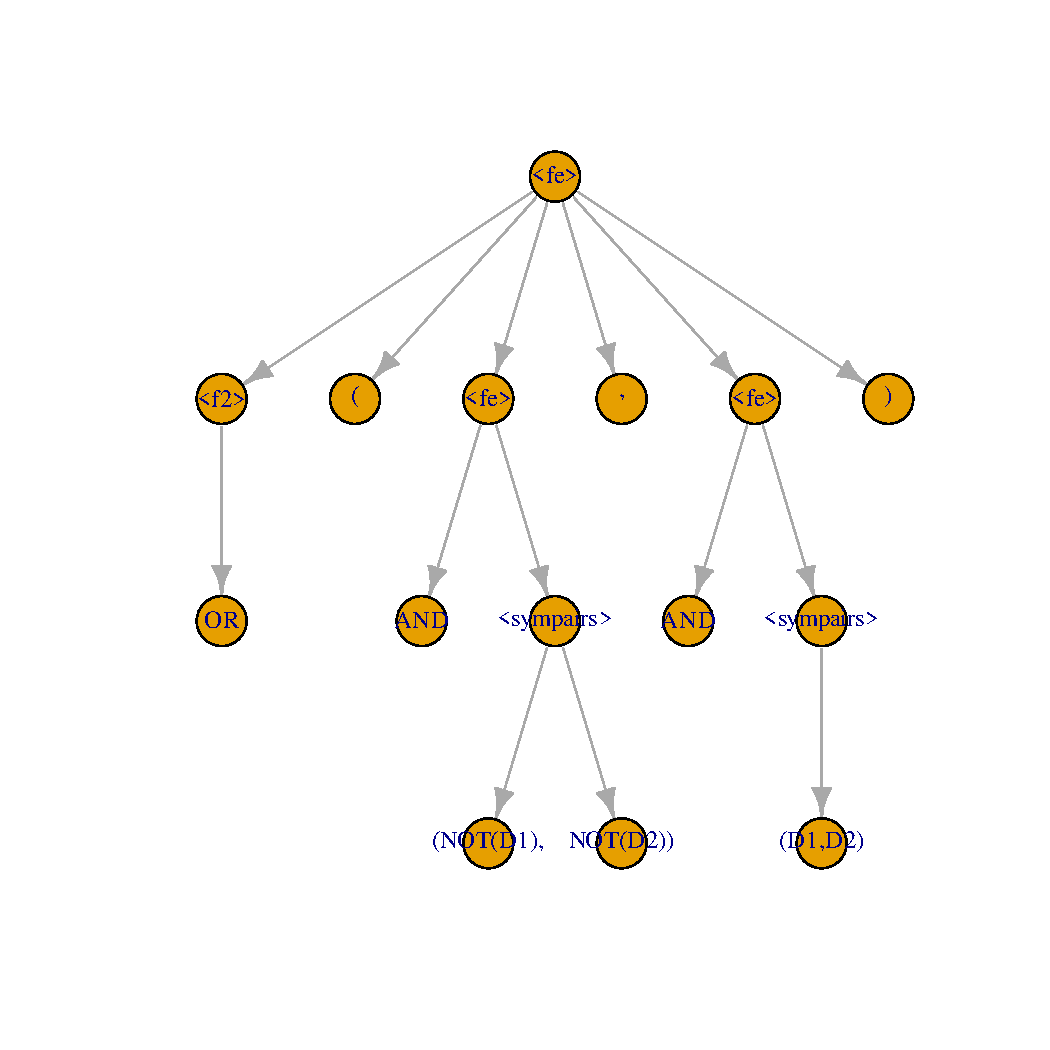
\includegraphics[width=0.5\textwidth, angle=0]
{ExpEDerivationTreeFigure000.pdf}
 \end{center}
 \label{report/ExpEDerivationTreeFigure000.pdf}  
 \end{frame}

% report/ExpEmain042.tex
% ExpE
% Figure: Plot of last xegaRun for Treatment BoolT4sgp2k of Experiment ExpE
% Thu May  8 17:40:54 2025
 \begin{frame}
 \frametitle{ Plot of last xegaRun for Treatment BoolT4sgp2k of Experiment ExpE }
 \begin{center}
\includegraphics[width=0.5\textwidth, angle=-90]
{ExpEPlotPopStatsFigure000.eps}
 \end{center}
 \label{report/ExpEPlotPopStatsFigure000.eps}  
 \end{frame}

% report/ExpEmain043.tex
\miniframesoff
\subsection{Treatment BoolT4sgp3k}
% report/ExpEmain044.tex
% ExpE
% Table:  Parameters of treatment: BoolT4sgp3k 

% Thu May  8 17:40:54 2025
 \begin{frame}
 \fontsize{8pt}{9pt}\selectfont
 \frametitle{  Parameters of treatment: BoolT4sgp3k 
 }
% latex table generated in R 4.4.3 by xtable 1.8-4 package
% Wed May 14 17:33:40 2025
\begin{table}[ht]
\centering
\begin{tabular}{rr}
  \hline
 & Parameter Values \\ 
  \hline
tRNG & L'Ecuyer-CMRG Inversion Rejection \\ 
  tReplay & 0 \\ 
  experimentName & EB \\ 
  treatmentName & BoolT4sgp3k \\ 
  trials & 20 \\ 
  everyK & 10 \\ 
  outpath & data \\ 
  batchPath & . \\ 
  tVerbose & 1 \\ 
   \hline
\end{tabular}
\caption{ Parameters of treatment: BoolT4sgp3k 
} 
\end{table}

 \label{ExpEtParmTable004.tex}  
 \end{frame}

 % Label:  \label{ExpEtParmTable004.tex}  
% report/ExpEmain045.tex
% ExpE
% Table:  Parameters of treatment BoolT4sgp3k passed to xegaRun

% Thu May  8 17:40:54 2025
 \begin{frame}
 \fontsize{8pt}{9pt}\selectfont
 \frametitle{  Parameters of treatment BoolT4sgp3k passed to xegaRun
 }
% latex table generated in R 4.4.3 by xtable 1.8-4 package
% Wed May 14 17:33:40 2025
\begin{table}[ht]
\centering
\begin{tabular}{rr}
  \hline
 & Parameter Values \\ 
  \hline
penv & 3-Symmetry Problem \\ 
  grammar & /home/dj2333/dev/cran/kSymmetry/BNF/AndOrNotTuned4.txt \\ 
  replay & 0 \\ 
  algorithm & sgp \\ 
  maxdepth & 7 \\ 
  max & FALSE \\ 
  worstFitness & -8 \\ 
  popsize & 200 \\ 
  generations & 500 \\ 
  crossrate & 0.2 \\ 
  mutrate & 0.4 \\ 
  ivmutrate & Const \\ 
  mutrate2 & 0.8 \\ 
  ivcrossrate & Const \\ 
  crossrate2 & 0.4 \\ 
   \hline
\end{tabular}
\caption{ Parameters of treatment BoolT4sgp3k passed to xegaRun
 (Part 1)} 
\end{table}

 \label{ExpEtParmTable005.tex}  
 \end{frame}

 % Label:  \label{ExpEtParmTable005.tex}  
% report/ExpEmain046.tex
% ExpE
% Table:  Parameters of treatment BoolT4sgp3k passed to xegaRun

% Thu May  8 17:40:54 2025
 \begin{frame}
 \fontsize{8pt}{9pt}\selectfont
 \frametitle{  Parameters of treatment BoolT4sgp3k passed to xegaRun
 }
% latex table generated in R 4.4.3 by xtable 1.8-4 package
% Thu May  8 17:40:54 2025
\begin{table}[ht]
\centering
\begin{tabular}{rr}
  \hline
 & Parameter Values \\ 
  \hline
scalefactor & Uniform \\ 
  genemap & Bin2Dec \\ 
  initgene & InitGene \\ 
  selection & SUS \\ 
  mateselection & SUS \\ 
  replication & Kid2 \\ 
  crossover & Cross2Gene \\ 
  mutation & MutateGene \\ 
  accept & All \\ 
  reportEvalErrors & TRUE \\ 
  codons & 120 \\ 
  codonPrecision & LCM \\ 
  terminationEps & -0.1 \\ 
  terminationCondition & AbsoluteError \\ 
  evalmethod & Deterministic \\ 
   \hline
\end{tabular}
\caption{ Parameters of treatment BoolT4sgp3k passed to xegaRun
 (Part 2)} 
\end{table}

 \label{ExpEtParmTable006.tex}  
 \end{frame}

 % Label:  \label{ExpEtParmTable006.tex}  
% report/ExpEmain047.tex
% ExpE
% Table:  Parameters of treatment BoolT4sgp3k passed to xegaRun

% Thu May  8 17:40:54 2025
 \begin{frame}
 \fontsize{8pt}{9pt}\selectfont
 \frametitle{  Parameters of treatment BoolT4sgp3k passed to xegaRun
 }
% latex table generated in R 4.4.3 by xtable 1.8-4 package
% Wed May 14 17:33:40 2025
\begin{table}[ht]
\centering
\begin{tabular}{rr}
  \hline
 & Parameter Values \\ 
  \hline
executionModel & MultiCore \\ 
  verbose & 1 \\ 
  batch & FALSE \\ 
  semantics & byValue \\ 
  path & . \\ 
   \hline
\end{tabular}
\caption{ Parameters of treatment BoolT4sgp3k passed to xegaRun
 (Part 3)} 
\end{table}

 \label{ExpEtParmTable007.tex}  
 \end{frame}

 % Label:  \label{ExpEtParmTable007.tex}  
% report/ExpEmain048.tex
% ExpE
% Table: The Production Table of Treatment BoolT4sgp3k of Experiment ExpE
% Thu May  8 17:40:54 2025
 \begin{frame}
 \fontsize{8pt}{9pt}\selectfont
 \frametitle{ The Production Table of Treatment BoolT4sgp3k of Experiment ExpE }
% latex table generated in R 4.4.3 by xtable 1.8-4 package
% Thu May  8 17:40:54 2025
\begin{table}[ht]
\centering
\begin{tabular}{rrr}
  \hline
 & LHS & RHS \\ 
  \hline
1 & $<$fe$>$ & $<$f0$>$ \\ 
  2 & $<$fe$>$ & $<$f1$>$($<$fe$>$) \\ 
  3 & $<$fe$>$ & $<$f2$>$($<$fe$>$,$<$fe$>$) \\ 
  4 & $<$f0$>$ & D1 \\ 
  5 & $<$f0$>$ & D2 \\ 
  6 & $<$f0$>$ & D3 \\ 
  7 & $<$fe$>$ & AND$<$sympairs$>$ \\ 
  8 & $<$fe$>$ & AND$<$sympairs$>$ \\ 
  9 & $<$sympairs$>$ & (D1,D3) \\ 
  10 & $<$sympairs$>$ & (NOT(D1),NOT(D3)) \\ 
  11 & $<$f1$>$ & NOT \\ 
  12 & $<$f2$>$ & OR \\ 
  13 & $<$f2$>$ & OR \\ 
  14 & $<$f2$>$ & AND \\ 
   \hline
\end{tabular}
\caption{The Production Table of Treatment BoolT4sgp3k of Experiment ExpE} 
\end{table}

 \label{ExpEGrammarTable001.tex}  
 \end{frame}

 % Label:  \label{ExpEGrammarTable001.tex}  
% report/ExpEmain049.tex
% ExpE
% Table: Treatment: BoolT4sgp3k
% Thu May  8 17:40:54 2025
 \begin{frame}
 \fontsize{8pt}{9pt}\selectfont
 \frametitle{ Treatment: BoolT4sgp3k }
% latex table generated in R 4.4.3 by xtable 1.8-4 package
% Wed May 14 17:33:41 2025
\begin{table}[ht]
\centering
\begin{tabular}{rrrrrrrr}
  \hline
 & Treatment & Trials & Variable & min & mean & sd & max \\ 
  \hline
8 & BoolT4sgp3k &  80 & Evaluations & 200.00 & 202.50 & 22.36 & 400.00 \\ 
  5 & BoolT4sgp3k &  80 & Fitness & 0.00 & 0.00 & 0.00 & 0.00 \\ 
  7 & BoolT4sgp3k &  80 & Generations & 1.00 & 1.01 & 0.11 & 2.00 \\ 
  6 & BoolT4sgp3k &  80 & Seconds & 0.21 & 0.30 & 0.06 & 0.68 \\ 
   \hline
\end{tabular}
\caption{Treatment: BoolT4sgp3k} 
\end{table}

 \label{ExpEStatsTable004.tex}  
 \end{frame}

 % Label:  \label{ExpEStatsTable004.tex}  
% report/ExpEmain050.tex
% ExpE
% Table: The Solution Table of Treatment BoolT4sgp3k of Experiment ExpE. Fit: 0. Unique Shortest Solutions: 28.
% Thu May  8 17:40:54 2025
 \begin{frame}
 \fontsize{8pt}{9pt}\selectfont
 \frametitle{ The Solution Table of Treatment BoolT4sgp3k of Experiment ExpE. Fit: 0. Unique Shortest Solutions: 28. }
% latex table generated in R 4.4.3 by xtable 1.8-4 package
% Wed May 14 17:33:41 2025
\begin{table}[ht]
\centering
\begin{tabular}{rp{9cm}}
  \hline
 & Solution \\ 
  \hline
1 & OR(AND(NOT(D1), NOT(D3)), AND(D1, D3)) \\ 
   \hline
\end{tabular}
\caption{The Solution Table of Treatment BoolT4sgp3k of Experiment ExpE. Fit: 0. Unique Shortest Solutions: 28.} 
\end{table}

 \label{ExpESolutionTable001.tex}  
 \end{frame}

 % Label:  \label{ExpESolutionTable001.tex}  
% report/ExpEmain051.tex
% ExpE
% Figure: The Derivation Tree of a Solution of Treatment BoolT4sgp3k of Experiment ExpE
% Thu May  8 17:40:54 2025
 \begin{frame}
 \frametitle{ The Derivation Tree of a Solution of Treatment BoolT4sgp3k of Experiment ExpE }
 \begin{center}
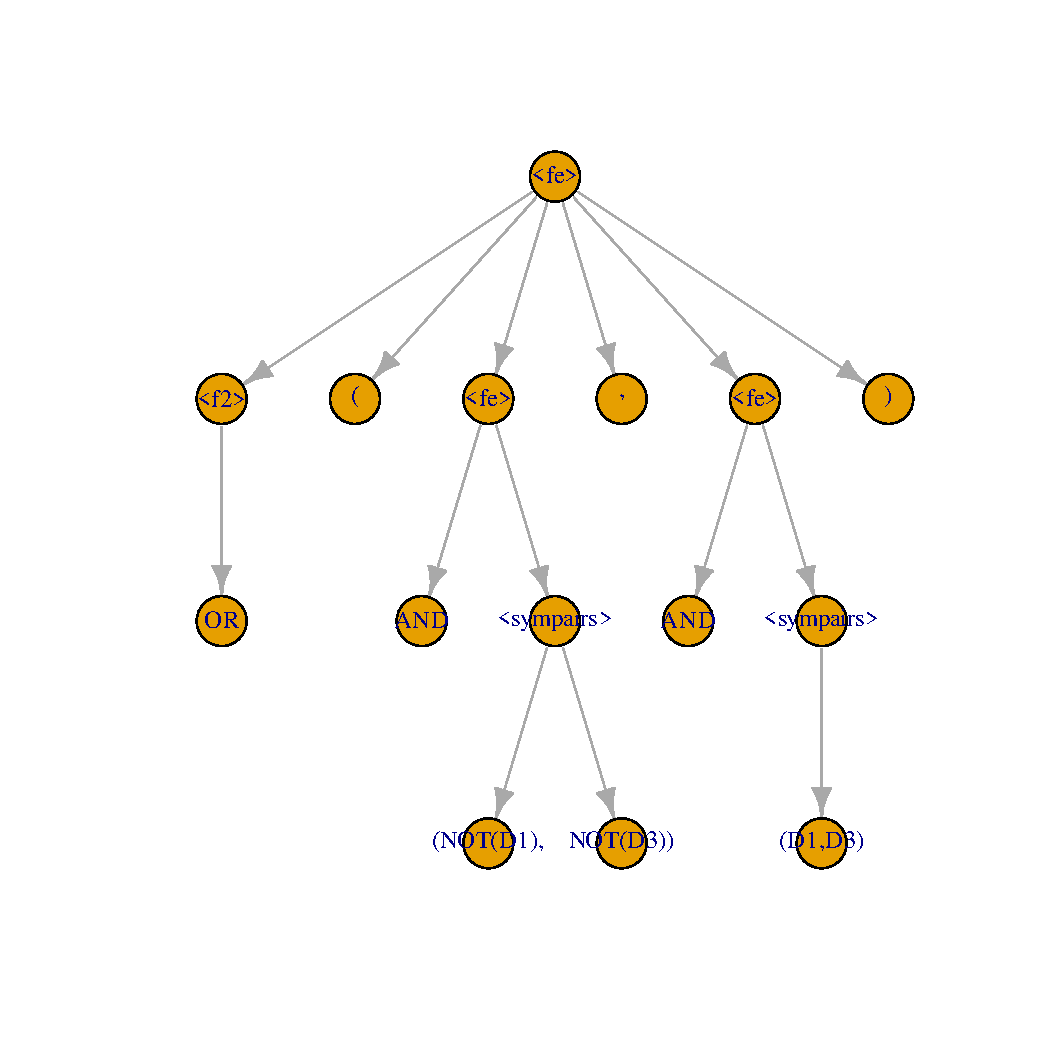
\includegraphics[width=0.5\textwidth, angle=0]
{ExpEDerivationTreeFigure001.pdf}
 \end{center}
 \label{report/ExpEDerivationTreeFigure001.pdf}  
 \end{frame}

% report/ExpEmain052.tex
% ExpE
% Figure: Plot of last xegaRun for Treatment BoolT4sgp3k of Experiment ExpE
% Thu May  8 17:40:54 2025
 \begin{frame}
 \frametitle{ Plot of last xegaRun for Treatment BoolT4sgp3k of Experiment ExpE }
 \begin{center}
\includegraphics[width=0.5\textwidth, angle=-90]
{ExpEPlotPopStatsFigure001.eps}
 \end{center}
 \label{report/ExpEPlotPopStatsFigure001.eps}  
 \end{frame}

% report/ExpEmain053.tex
\miniframesoff
\subsection{Treatment BoolT4sgp4k}
% report/ExpEmain054.tex
% ExpE
% Table:  Parameters of treatment: BoolT4sgp4k 

% Thu May  8 17:40:54 2025
 \begin{frame}
 \fontsize{8pt}{9pt}\selectfont
 \frametitle{  Parameters of treatment: BoolT4sgp4k 
 }
% latex table generated in R 4.4.3 by xtable 1.8-4 package
% Thu May  8 17:40:54 2025
\begin{table}[ht]
\centering
\begin{tabular}{rr}
  \hline
 & Parameter Values \\ 
  \hline
tRNG & L'Ecuyer-CMRG Inversion Rejection \\ 
  tReplay & 0 \\ 
  experimentName & EB \\ 
  treatmentName & BoolT4sgp4k \\ 
  trials & 20 \\ 
  everyK & 10 \\ 
  outpath & data \\ 
  batchPath & . \\ 
  tVerbose & 1 \\ 
   \hline
\end{tabular}
\caption{ Parameters of treatment: BoolT4sgp4k 
} 
\end{table}

 \label{ExpEtParmTable008.tex}  
 \end{frame}

 % Label:  \label{ExpEtParmTable008.tex}  
% report/ExpEmain055.tex
% ExpE
% Table:  Parameters of treatment BoolT4sgp4k passed to xegaRun

% Thu May  8 17:40:54 2025
 \begin{frame}
 \fontsize{8pt}{9pt}\selectfont
 \frametitle{  Parameters of treatment BoolT4sgp4k passed to xegaRun
 }
% latex table generated in R 4.4.3 by xtable 1.8-4 package
% Thu May  8 17:40:54 2025
\begin{table}[ht]
\centering
\begin{tabular}{rr}
  \hline
 & Parameter Values \\ 
  \hline
penv & 4-Symmetry Problem \\ 
  grammar & /home/dj2333/dev/cran/kSymmetry/BNF/AndOrNotTuned4.txt \\ 
  replay & 0 \\ 
  algorithm & sgp \\ 
  maxdepth & 7 \\ 
  max & FALSE \\ 
  worstFitness & -16 \\ 
  popsize & 200 \\ 
  generations & 500 \\ 
  crossrate & 0.2 \\ 
  mutrate & 0.4 \\ 
  ivmutrate & Const \\ 
  mutrate2 & 0.8 \\ 
  ivcrossrate & Const \\ 
  crossrate2 & 0.4 \\ 
   \hline
\end{tabular}
\caption{ Parameters of treatment BoolT4sgp4k passed to xegaRun
 (Part 1)} 
\end{table}

 \label{ExpEtParmTable009.tex}  
 \end{frame}

 % Label:  \label{ExpEtParmTable009.tex}  
% report/ExpEmain056.tex
% ExpE
% Table:  Parameters of treatment BoolT4sgp4k passed to xegaRun

% Thu May  8 17:40:54 2025
 \begin{frame}
 \fontsize{8pt}{9pt}\selectfont
 \frametitle{  Parameters of treatment BoolT4sgp4k passed to xegaRun
 }
% latex table generated in R 4.4.3 by xtable 1.8-4 package
% Wed May 14 17:33:41 2025
\begin{table}[ht]
\centering
\begin{tabular}{rr}
  \hline
 & Parameter Values \\ 
  \hline
scalefactor & Uniform \\ 
  genemap & Bin2Dec \\ 
  initgene & InitGene \\ 
  selection & SUS \\ 
  mateselection & SUS \\ 
  replication & Kid2 \\ 
  crossover & Cross2Gene \\ 
  mutation & MutateGene \\ 
  accept & All \\ 
  reportEvalErrors & TRUE \\ 
  codons & 160 \\ 
  codonPrecision & LCM \\ 
  terminationEps & -0.1 \\ 
  terminationCondition & AbsoluteError \\ 
  evalmethod & Deterministic \\ 
   \hline
\end{tabular}
\caption{ Parameters of treatment BoolT4sgp4k passed to xegaRun
 (Part 2)} 
\end{table}

 \label{ExpEtParmTable010.tex}  
 \end{frame}

 % Label:  \label{ExpEtParmTable010.tex}  
% report/ExpEmain057.tex
% ExpE
% Table:  Parameters of treatment BoolT4sgp4k passed to xegaRun

% Thu May  8 17:40:54 2025
 \begin{frame}
 \fontsize{8pt}{9pt}\selectfont
 \frametitle{  Parameters of treatment BoolT4sgp4k passed to xegaRun
 }
% latex table generated in R 4.4.3 by xtable 1.8-4 package
% Wed May 14 17:33:41 2025
\begin{table}[ht]
\centering
\begin{tabular}{rr}
  \hline
 & Parameter Values \\ 
  \hline
executionModel & MultiCore \\ 
  verbose & 1 \\ 
  batch & FALSE \\ 
  semantics & byValue \\ 
  path & . \\ 
   \hline
\end{tabular}
\caption{ Parameters of treatment BoolT4sgp4k passed to xegaRun
 (Part 3)} 
\end{table}

 \label{ExpEtParmTable011.tex}  
 \end{frame}

 % Label:  \label{ExpEtParmTable011.tex}  
% report/ExpEmain058.tex
% ExpE
% Table: The Production Table of Treatment BoolT4sgp4k of Experiment ExpE
% Thu May  8 17:40:54 2025
 \begin{frame}
 \fontsize{8pt}{9pt}\selectfont
 \frametitle{ The Production Table of Treatment BoolT4sgp4k of Experiment ExpE }
% latex table generated in R 4.4.3 by xtable 1.8-4 package
% Thu May  8 17:40:54 2025
\begin{table}[ht]
\centering
\begin{tabular}{rrr}
  \hline
 & LHS & RHS \\ 
  \hline
1 & $<$fe$>$ & $<$f0$>$ \\ 
  2 & $<$fe$>$ & $<$f1$>$($<$fe$>$) \\ 
  3 & $<$fe$>$ & $<$f2$>$($<$fe$>$,$<$fe$>$) \\ 
  4 & $<$f0$>$ & D1 \\ 
  5 & $<$f0$>$ & D2 \\ 
  6 & $<$f0$>$ & D3 \\ 
  7 & $<$f0$>$ & D4 \\ 
  8 & $<$fe$>$ & AND$<$sympairs$>$ \\ 
  9 & $<$fe$>$ & AND$<$sympairs$>$ \\ 
  10 & $<$sympairs$>$ & (D1,D4) \\ 
  11 & $<$sympairs$>$ & (NOT(D1),NOT(D4)) \\ 
  12 & $<$sympairs$>$ & (D2,D3) \\ 
  13 & $<$sympairs$>$ & (NOT(D2),NOT(D3)) \\ 
  14 & $<$f1$>$ & NOT \\ 
  15 & $<$f2$>$ & OR \\ 
   \hline
\end{tabular}
\caption{The Production Table of Treatment BoolT4sgp4k of Experiment ExpE (Part 1)} 
\end{table}

 \label{ExpEGrammarTable002.tex}  
 \end{frame}

 % Label:  \label{ExpEGrammarTable002.tex}  
% report/ExpEmain059.tex
% ExpE
% Table: The Production Table of Treatment BoolT4sgp4k of Experiment ExpE
% Thu May  8 17:40:54 2025
 \begin{frame}
 \fontsize{8pt}{9pt}\selectfont
 \frametitle{ The Production Table of Treatment BoolT4sgp4k of Experiment ExpE }
% latex table generated in R 4.4.3 by xtable 1.8-4 package
% Thu May  8 17:40:54 2025
\begin{table}[ht]
\centering
\begin{tabular}{rrr}
  \hline
 & LHS & RHS \\ 
  \hline
16 & $<$f2$>$ & OR \\ 
  17 & $<$f2$>$ & AND \\ 
   \hline
\end{tabular}
\caption{The Production Table of Treatment BoolT4sgp4k of Experiment ExpE (Part 2)} 
\end{table}

 \label{ExpEGrammarTable003.tex}  
 \end{frame}

 % Label:  \label{ExpEGrammarTable003.tex}  
% report/ExpEmain060.tex
% ExpE
% Table: Treatment: BoolT4sgp4k
% Thu May  8 17:40:54 2025
 \begin{frame}
 \fontsize{8pt}{9pt}\selectfont
 \frametitle{ Treatment: BoolT4sgp4k }
% latex table generated in R 4.4.3 by xtable 1.8-4 package
% Wed May 14 17:33:41 2025
\begin{table}[ht]
\centering
\begin{tabular}{rrrrrrrr}
  \hline
 & Treatment & Trials & Variable & min & mean & sd & max \\ 
  \hline
12 & BoolT4sgp4k &  80 & Evaluations & 1400.00 & 15402.50 & 8377.03 & 44200.00 \\ 
  9 & BoolT4sgp4k &  80 & Fitness & 0.00 & 0.00 & 0.00 & 0.00 \\ 
  11 & BoolT4sgp4k &  80 & Generations & 7.00 & 77.01 & 41.89 & 221.00 \\ 
  10 & BoolT4sgp4k &  80 & Seconds & 1.32 & 17.93 & 11.89 & 71.35 \\ 
   \hline
\end{tabular}
\caption{Treatment: BoolT4sgp4k} 
\end{table}

 \label{ExpEStatsTable005.tex}  
 \end{frame}

 % Label:  \label{ExpEStatsTable005.tex}  
% report/ExpEmain061.tex
% ExpE
% Table: The Solution Table of Treatment BoolT4sgp4k of Experiment ExpE. Fit: 0. Unique Shortest Solutions: 68.
% Thu May  8 17:40:54 2025
 \begin{frame}
 \fontsize{8pt}{9pt}\selectfont
 \frametitle{ The Solution Table of Treatment BoolT4sgp4k of Experiment ExpE. Fit: 0. Unique Shortest Solutions: 68. }
% latex table generated in R 4.4.3 by xtable 1.8-4 package
% Wed May 14 17:33:41 2025
\begin{table}[ht]
\centering
\begin{tabular}{rp{9cm}}
  \hline
 & Solution \\ 
  \hline
1 & AND(OR(AND(NOT(D2), NOT(D3)), AND(D2, D3)), OR(AND(D1, D4), AND(NOT(D1), NOT(D4)))) \\ 
   \hline
\end{tabular}
\caption{The Solution Table of Treatment BoolT4sgp4k of Experiment ExpE. Fit: 0. Unique Shortest Solutions: 68.} 
\end{table}

 \label{ExpESolutionTable002.tex}  
 \end{frame}

 % Label:  \label{ExpESolutionTable002.tex}  
% report/ExpEmain062.tex
% ExpE
% Figure: The Derivation Tree of a Solution of Treatment BoolT4sgp4k of Experiment ExpE
% Thu May  8 17:40:54 2025
 \begin{frame}
 \frametitle{ The Derivation Tree of a Solution of Treatment BoolT4sgp4k of Experiment ExpE }
 \begin{center}
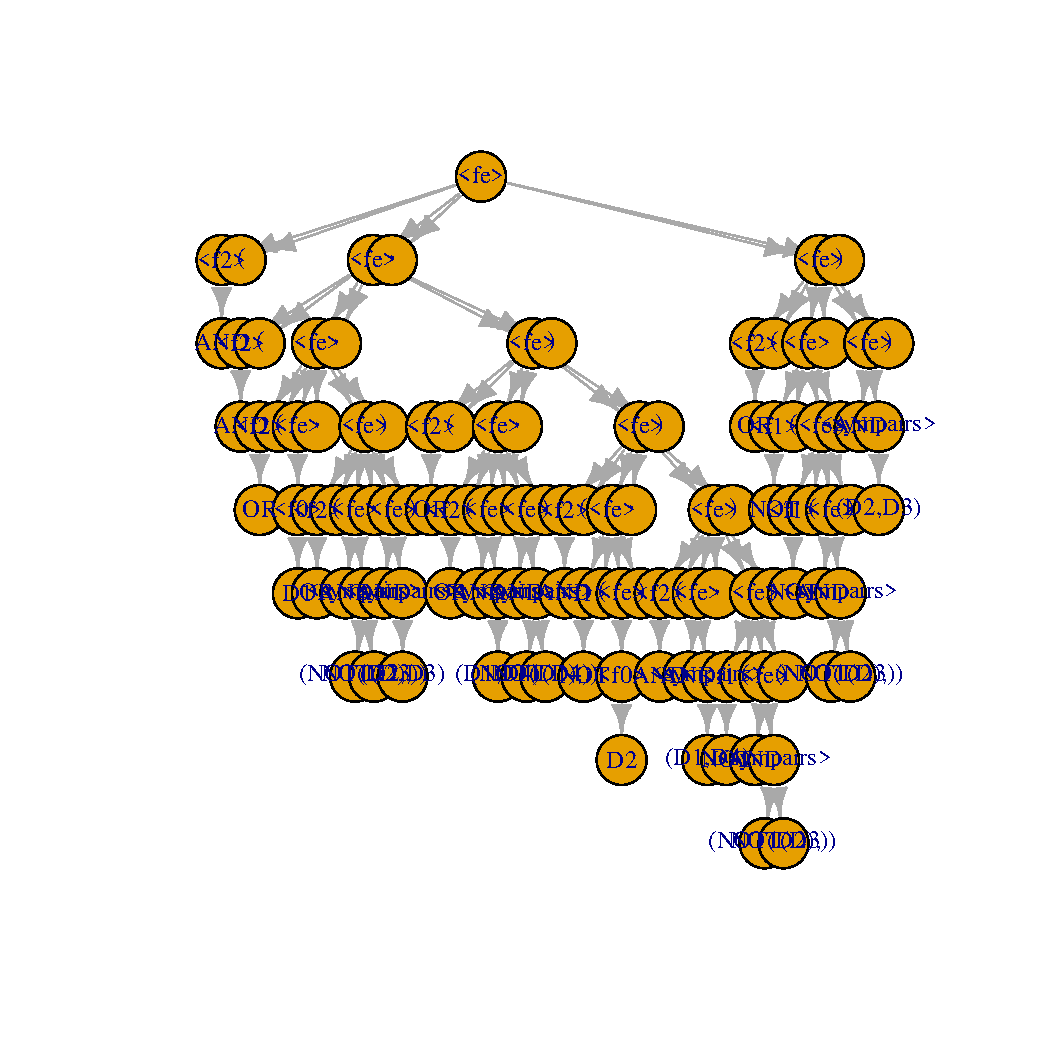
\includegraphics[width=0.5\textwidth, angle=0]
{ExpEDerivationTreeFigure002.pdf}
 \end{center}
 \label{report/ExpEDerivationTreeFigure002.pdf}  
 \end{frame}

% report/ExpEmain063.tex
% ExpE
% Figure: Plot of last xegaRun for Treatment BoolT4sgp4k of Experiment ExpE
% Thu May  8 17:40:54 2025
 \begin{frame}
 \frametitle{ Plot of last xegaRun for Treatment BoolT4sgp4k of Experiment ExpE }
 \begin{center}
\includegraphics[width=0.5\textwidth, angle=-90]
{ExpEPlotPopStatsFigure002.eps}
 \end{center}
 \label{report/ExpEPlotPopStatsFigure002.eps}  
 \end{frame}

% report/ExpEmain064.tex
\miniframesoff
\subsection{Treatment BoolT4sgp5k}
% report/ExpEmain065.tex
% ExpE
% Table:  Parameters of treatment: BoolT4sgp5k 

% Thu May  8 17:40:54 2025
 \begin{frame}
 \fontsize{8pt}{9pt}\selectfont
 \frametitle{  Parameters of treatment: BoolT4sgp5k 
 }
% latex table generated in R 4.4.3 by xtable 1.8-4 package
% Thu May  8 17:40:54 2025
\begin{table}[ht]
\centering
\begin{tabular}{rr}
  \hline
 & Parameter Values \\ 
  \hline
tRNG & L'Ecuyer-CMRG Inversion Rejection \\ 
  tReplay & 0 \\ 
  experimentName & EB \\ 
  treatmentName & BoolT4sgp5k \\ 
  trials & 20 \\ 
  everyK & 10 \\ 
  outpath & data \\ 
  batchPath & . \\ 
  tVerbose & 1 \\ 
   \hline
\end{tabular}
\caption{ Parameters of treatment: BoolT4sgp5k 
} 
\end{table}

 \label{ExpEtParmTable012.tex}  
 \end{frame}

 % Label:  \label{ExpEtParmTable012.tex}  
% report/ExpEmain066.tex
% ExpE
% Table:  Parameters of treatment BoolT4sgp5k passed to xegaRun

% Thu May  8 17:40:54 2025
 \begin{frame}
 \fontsize{8pt}{9pt}\selectfont
 \frametitle{  Parameters of treatment BoolT4sgp5k passed to xegaRun
 }
% latex table generated in R 4.4.3 by xtable 1.8-4 package
% Wed May 14 17:33:41 2025
\begin{table}[ht]
\centering
\begin{tabular}{rr}
  \hline
 & Parameter Values \\ 
  \hline
penv & 5-Symmetry Problem \\ 
  grammar & /home/dj2333/dev/cran/kSymmetry/BNF/AndOrNotTuned4.txt \\ 
  replay & 0 \\ 
  algorithm & sgp \\ 
  maxdepth & 7 \\ 
  max & FALSE \\ 
  worstFitness & -32 \\ 
  popsize & 200 \\ 
  generations & 500 \\ 
  crossrate & 0.2 \\ 
  mutrate & 0.4 \\ 
  ivmutrate & Const \\ 
  mutrate2 & 0.8 \\ 
  ivcrossrate & Const \\ 
  crossrate2 & 0.4 \\ 
   \hline
\end{tabular}
\caption{ Parameters of treatment BoolT4sgp5k passed to xegaRun
 (Part 1)} 
\end{table}

 \label{ExpEtParmTable013.tex}  
 \end{frame}

 % Label:  \label{ExpEtParmTable013.tex}  
% report/ExpEmain067.tex
% ExpE
% Table:  Parameters of treatment BoolT4sgp5k passed to xegaRun

% Thu May  8 17:40:54 2025
 \begin{frame}
 \fontsize{8pt}{9pt}\selectfont
 \frametitle{  Parameters of treatment BoolT4sgp5k passed to xegaRun
 }
% latex table generated in R 4.4.3 by xtable 1.8-4 package
% Wed May 14 17:33:41 2025
\begin{table}[ht]
\centering
\begin{tabular}{rr}
  \hline
 & Parameter Values \\ 
  \hline
scalefactor & Uniform \\ 
  genemap & Bin2Dec \\ 
  initgene & InitGene \\ 
  selection & SUS \\ 
  mateselection & SUS \\ 
  replication & Kid2 \\ 
  crossover & Cross2Gene \\ 
  mutation & MutateGene \\ 
  accept & All \\ 
  reportEvalErrors & TRUE \\ 
  codons & 200 \\ 
  codonPrecision & LCM \\ 
  terminationEps & -0.1 \\ 
  terminationCondition & AbsoluteError \\ 
  evalmethod & Deterministic \\ 
   \hline
\end{tabular}
\caption{ Parameters of treatment BoolT4sgp5k passed to xegaRun
 (Part 2)} 
\end{table}

 \label{ExpEtParmTable014.tex}  
 \end{frame}

 % Label:  \label{ExpEtParmTable014.tex}  
% report/ExpEmain068.tex
% ExpE
% Table:  Parameters of treatment BoolT4sgp5k passed to xegaRun

% Thu May  8 17:40:54 2025
 \begin{frame}
 \fontsize{8pt}{9pt}\selectfont
 \frametitle{  Parameters of treatment BoolT4sgp5k passed to xegaRun
 }
% latex table generated in R 4.4.3 by xtable 1.8-4 package
% Wed May 14 17:33:41 2025
\begin{table}[ht]
\centering
\begin{tabular}{rr}
  \hline
 & Parameter Values \\ 
  \hline
executionModel & MultiCore \\ 
  verbose & 1 \\ 
  batch & FALSE \\ 
  semantics & byValue \\ 
  path & . \\ 
   \hline
\end{tabular}
\caption{ Parameters of treatment BoolT4sgp5k passed to xegaRun
 (Part 3)} 
\end{table}

 \label{ExpEtParmTable015.tex}  
 \end{frame}

 % Label:  \label{ExpEtParmTable015.tex}  
% report/ExpEmain069.tex
% ExpE
% Table: The Production Table of Treatment BoolT4sgp5k of Experiment ExpE
% Thu May  8 17:40:54 2025
 \begin{frame}
 \fontsize{8pt}{9pt}\selectfont
 \frametitle{ The Production Table of Treatment BoolT4sgp5k of Experiment ExpE }
% latex table generated in R 4.4.3 by xtable 1.8-4 package
% Thu May  8 17:40:54 2025
\begin{table}[ht]
\centering
\begin{tabular}{rrr}
  \hline
 & LHS & RHS \\ 
  \hline
1 & $<$fe$>$ & $<$f0$>$ \\ 
  2 & $<$fe$>$ & $<$f1$>$($<$fe$>$) \\ 
  3 & $<$fe$>$ & $<$f2$>$($<$fe$>$,$<$fe$>$) \\ 
  4 & $<$f0$>$ & D1 \\ 
  5 & $<$f0$>$ & D2 \\ 
  6 & $<$f0$>$ & D3 \\ 
  7 & $<$f0$>$ & D4 \\ 
  8 & $<$f0$>$ & D5 \\ 
  9 & $<$fe$>$ & AND$<$sympairs$>$ \\ 
  10 & $<$fe$>$ & AND$<$sympairs$>$ \\ 
  11 & $<$sympairs$>$ & (D1,D5) \\ 
  12 & $<$sympairs$>$ & (NOT(D1),NOT(D5)) \\ 
  13 & $<$sympairs$>$ & (D2,D4) \\ 
  14 & $<$sympairs$>$ & (NOT(D2),NOT(D4)) \\ 
  15 & $<$f1$>$ & NOT \\ 
   \hline
\end{tabular}
\caption{The Production Table of Treatment BoolT4sgp5k of Experiment ExpE (Part 1)} 
\end{table}

 \label{ExpEGrammarTable004.tex}  
 \end{frame}

 % Label:  \label{ExpEGrammarTable004.tex}  
% report/ExpEmain070.tex
% ExpE
% Table: The Production Table of Treatment BoolT4sgp5k of Experiment ExpE
% Thu May  8 17:40:54 2025
 \begin{frame}
 \fontsize{8pt}{9pt}\selectfont
 \frametitle{ The Production Table of Treatment BoolT4sgp5k of Experiment ExpE }
% latex table generated in R 4.4.3 by xtable 1.8-4 package
% Wed May 14 17:33:41 2025
\begin{table}[ht]
\centering
\begin{tabular}{rrr}
  \hline
 & LHS & RHS \\ 
  \hline
16 & $<$f2$>$ & OR \\ 
  17 & $<$f2$>$ & OR \\ 
  18 & $<$f2$>$ & AND \\ 
   \hline
\end{tabular}
\caption{The Production Table of Treatment BoolT4sgp5k of Experiment ExpE (Part 2)} 
\end{table}

 \label{ExpEGrammarTable005.tex}  
 \end{frame}

 % Label:  \label{ExpEGrammarTable005.tex}  
% report/ExpEmain071.tex
% ExpE
% Table: Treatment: BoolT4sgp5k
% Thu May  8 17:40:54 2025
 \begin{frame}
 \fontsize{8pt}{9pt}\selectfont
 \frametitle{ Treatment: BoolT4sgp5k }
% latex table generated in R 4.4.3 by xtable 1.8-4 package
% Wed May 14 17:33:41 2025
\begin{table}[ht]
\centering
\begin{tabular}{rrrrrrrr}
  \hline
 & Treatment & Trials & Variable & min & mean & sd & max \\ 
  \hline
16 & BoolT4sgp5k &  80 & Evaluations & 2000.00 & 14620.00 & 10549.35 & 51200.00 \\ 
  13 & BoolT4sgp5k &  80 & Fitness & 0.00 & 0.00 & 0.00 & 0.00 \\ 
  15 & BoolT4sgp5k &  80 & Generations & 10.00 & 73.10 & 52.75 & 256.00 \\ 
  14 & BoolT4sgp5k &  80 & Seconds & 1.50 & 18.16 & 17.35 & 103.10 \\ 
   \hline
\end{tabular}
\caption{Treatment: BoolT4sgp5k} 
\end{table}

 \label{ExpEStatsTable006.tex}  
 \end{frame}

 % Label:  \label{ExpEStatsTable006.tex}  
% report/ExpEmain072.tex
% ExpE
% Table: The Solution Table of Treatment BoolT4sgp5k of Experiment ExpE. Fit: 0. Unique Shortest Solutions: 71.
% Thu May  8 17:40:54 2025
 \begin{frame}
 \fontsize{8pt}{9pt}\selectfont
 \frametitle{ The Solution Table of Treatment BoolT4sgp5k of Experiment ExpE. Fit: 0. Unique Shortest Solutions: 71. }
% latex table generated in R 4.4.3 by xtable 1.8-4 package
% Thu May  8 17:40:54 2025
\begin{table}[ht]
\centering
\begin{tabular}{rp{9cm}}
  \hline
 & Solution \\ 
  \hline
1 & AND(OR(AND(NOT(D2), NOT(D4)), AND(D2, D4)), OR(AND(NOT(D1), NOT(D5)), AND(D1, D5))) \\ 
   \hline
\end{tabular}
\caption{The Solution Table of Treatment BoolT4sgp5k of Experiment ExpE. Fit: 0. Unique Shortest Solutions: 71.} 
\end{table}

 \label{ExpESolutionTable003.tex}  
 \end{frame}

 % Label:  \label{ExpESolutionTable003.tex}  
% report/ExpEmain073.tex
% ExpE
% Figure: The Derivation Tree of a Solution of Treatment BoolT4sgp5k of Experiment ExpE
% Thu May  8 17:40:54 2025
 \begin{frame}
 \frametitle{ The Derivation Tree of a Solution of Treatment BoolT4sgp5k of Experiment ExpE }
 \begin{center}
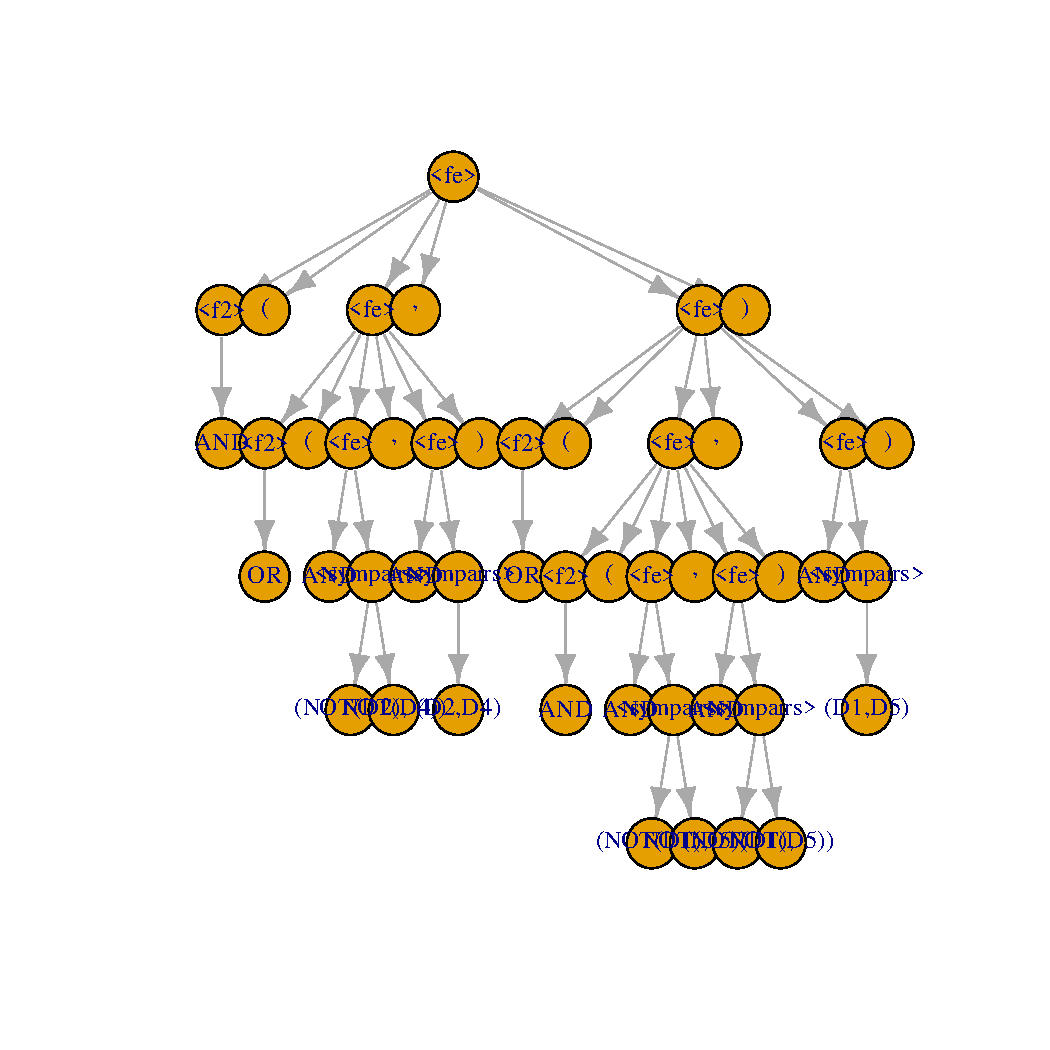
\includegraphics[width=0.5\textwidth, angle=0]
{ExpEDerivationTreeFigure003.pdf}
 \end{center}
 \label{report/ExpEDerivationTreeFigure003.pdf}  
 \end{frame}

% report/ExpEmain074.tex
% ExpE
% Figure: Plot of last xegaRun for Treatment BoolT4sgp5k of Experiment ExpE
% Thu May  8 17:40:54 2025
 \begin{frame}
 \frametitle{ Plot of last xegaRun for Treatment BoolT4sgp5k of Experiment ExpE }
 \begin{center}
\includegraphics[width=0.5\textwidth, angle=-90]
{ExpEPlotPopStatsFigure003.eps}
 \end{center}
 \label{report/ExpEPlotPopStatsFigure003.eps}  
 \end{frame}

% report/ExpEmain075.tex
\miniframesoff
\subsection{Treatment BoolT4sgp6k}
% report/ExpEmain076.tex
% ExpE
% Table:  Parameters of treatment: BoolT4sgp6k 

% Thu May  8 17:40:54 2025
 \begin{frame}
 \fontsize{8pt}{9pt}\selectfont
 \frametitle{  Parameters of treatment: BoolT4sgp6k 
 }
% latex table generated in R 4.4.3 by xtable 1.8-4 package
% Wed May 14 17:33:41 2025
\begin{table}[ht]
\centering
\begin{tabular}{rr}
  \hline
 & Parameter Values \\ 
  \hline
tRNG & L'Ecuyer-CMRG Inversion Rejection \\ 
  tReplay & 0 \\ 
  experimentName & EB \\ 
  treatmentName & BoolT4sgp6k \\ 
  trials & 20 \\ 
  everyK & 10 \\ 
  outpath & data \\ 
  batchPath & . \\ 
  tVerbose & 1 \\ 
   \hline
\end{tabular}
\caption{ Parameters of treatment: BoolT4sgp6k 
} 
\end{table}

 \label{ExpEtParmTable016.tex}  
 \end{frame}

 % Label:  \label{ExpEtParmTable016.tex}  
% report/ExpEmain077.tex
% ExpE
% Table:  Parameters of treatment BoolT4sgp6k passed to xegaRun

% Thu May  8 17:40:54 2025
 \begin{frame}
 \fontsize{8pt}{9pt}\selectfont
 \frametitle{  Parameters of treatment BoolT4sgp6k passed to xegaRun
 }
% latex table generated in R 4.4.3 by xtable 1.8-4 package
% Wed May 14 17:33:41 2025
\begin{table}[ht]
\centering
\begin{tabular}{rr}
  \hline
 & Parameter Values \\ 
  \hline
penv & 6-Symmetry Problem \\ 
  grammar & /home/dj2333/dev/cran/kSymmetry/BNF/AndOrNotTuned4.txt \\ 
  replay & 0 \\ 
  algorithm & sgp \\ 
  maxdepth & 7 \\ 
  max & FALSE \\ 
  worstFitness & -64 \\ 
  popsize & 200 \\ 
  generations & 500 \\ 
  crossrate & 0.2 \\ 
  mutrate & 0.4 \\ 
  ivmutrate & Const \\ 
  mutrate2 & 0.8 \\ 
  ivcrossrate & Const \\ 
  crossrate2 & 0.4 \\ 
   \hline
\end{tabular}
\caption{ Parameters of treatment BoolT4sgp6k passed to xegaRun
 (Part 1)} 
\end{table}

 \label{ExpEtParmTable017.tex}  
 \end{frame}

 % Label:  \label{ExpEtParmTable017.tex}  
% report/ExpEmain078.tex
% ExpE
% Table:  Parameters of treatment BoolT4sgp6k passed to xegaRun

% Thu May  8 17:40:54 2025
 \begin{frame}
 \fontsize{8pt}{9pt}\selectfont
 \frametitle{  Parameters of treatment BoolT4sgp6k passed to xegaRun
 }
% latex table generated in R 4.4.3 by xtable 1.8-4 package
% Wed May 14 17:33:41 2025
\begin{table}[ht]
\centering
\begin{tabular}{rr}
  \hline
 & Parameter Values \\ 
  \hline
scalefactor & Uniform \\ 
  genemap & Bin2Dec \\ 
  initgene & InitGene \\ 
  selection & SUS \\ 
  mateselection & SUS \\ 
  replication & Kid2 \\ 
  crossover & Cross2Gene \\ 
  mutation & MutateGene \\ 
  accept & All \\ 
  reportEvalErrors & TRUE \\ 
  codons & 240 \\ 
  codonPrecision & LCM \\ 
  terminationEps & -0.1 \\ 
  terminationCondition & AbsoluteError \\ 
  evalmethod & Deterministic \\ 
   \hline
\end{tabular}
\caption{ Parameters of treatment BoolT4sgp6k passed to xegaRun
 (Part 2)} 
\end{table}

 \label{ExpEtParmTable018.tex}  
 \end{frame}

 % Label:  \label{ExpEtParmTable018.tex}  
% report/ExpEmain079.tex
% ExpE
% Table:  Parameters of treatment BoolT4sgp6k passed to xegaRun

% Thu May  8 17:40:54 2025
 \begin{frame}
 \fontsize{8pt}{9pt}\selectfont
 \frametitle{  Parameters of treatment BoolT4sgp6k passed to xegaRun
 }
% latex table generated in R 4.4.3 by xtable 1.8-4 package
% Wed May 14 17:33:41 2025
\begin{table}[ht]
\centering
\begin{tabular}{rr}
  \hline
 & Parameter Values \\ 
  \hline
executionModel & MultiCore \\ 
  verbose & 1 \\ 
  batch & FALSE \\ 
  semantics & byValue \\ 
  path & . \\ 
   \hline
\end{tabular}
\caption{ Parameters of treatment BoolT4sgp6k passed to xegaRun
 (Part 3)} 
\end{table}

 \label{ExpEtParmTable019.tex}  
 \end{frame}

 % Label:  \label{ExpEtParmTable019.tex}  
% report/ExpEmain080.tex
% ExpE
% Table: The Production Table of Treatment BoolT4sgp6k of Experiment ExpE
% Thu May  8 17:40:54 2025
 \begin{frame}
 \fontsize{8pt}{9pt}\selectfont
 \frametitle{ The Production Table of Treatment BoolT4sgp6k of Experiment ExpE }
% latex table generated in R 4.4.3 by xtable 1.8-4 package
% Thu May  8 17:40:54 2025
\begin{table}[ht]
\centering
\begin{tabular}{rrr}
  \hline
 & LHS & RHS \\ 
  \hline
1 & $<$fe$>$ & $<$f0$>$ \\ 
  2 & $<$fe$>$ & $<$f1$>$($<$fe$>$) \\ 
  3 & $<$fe$>$ & $<$f2$>$($<$fe$>$,$<$fe$>$) \\ 
  4 & $<$f0$>$ & D1 \\ 
  5 & $<$f0$>$ & D2 \\ 
  6 & $<$f0$>$ & D3 \\ 
  7 & $<$f0$>$ & D4 \\ 
  8 & $<$f0$>$ & D5 \\ 
  9 & $<$f0$>$ & D6 \\ 
  10 & $<$fe$>$ & AND$<$sympairs$>$ \\ 
  11 & $<$fe$>$ & AND$<$sympairs$>$ \\ 
  12 & $<$sympairs$>$ & (D1,D6) \\ 
  13 & $<$sympairs$>$ & (NOT(D1),NOT(D6)) \\ 
  14 & $<$sympairs$>$ & (D2,D5) \\ 
  15 & $<$sympairs$>$ & (NOT(D2),NOT(D5)) \\ 
   \hline
\end{tabular}
\caption{The Production Table of Treatment BoolT4sgp6k of Experiment ExpE (Part 1)} 
\end{table}

 \label{ExpEGrammarTable006.tex}  
 \end{frame}

 % Label:  \label{ExpEGrammarTable006.tex}  
% report/ExpEmain081.tex
% ExpE
% Table: The Production Table of Treatment BoolT4sgp6k of Experiment ExpE
% Thu May  8 17:40:54 2025
 \begin{frame}
 \fontsize{8pt}{9pt}\selectfont
 \frametitle{ The Production Table of Treatment BoolT4sgp6k of Experiment ExpE }
% latex table generated in R 4.4.3 by xtable 1.8-4 package
% Wed May 14 17:33:41 2025
\begin{table}[ht]
\centering
\begin{tabular}{rrr}
  \hline
 & LHS & RHS \\ 
  \hline
16 & $<$sympairs$>$ & (D3,D4) \\ 
  17 & $<$sympairs$>$ & (NOT(D3),NOT(D4)) \\ 
  18 & $<$f1$>$ & NOT \\ 
  19 & $<$f2$>$ & OR \\ 
  20 & $<$f2$>$ & OR \\ 
  21 & $<$f2$>$ & AND \\ 
   \hline
\end{tabular}
\caption{The Production Table of Treatment BoolT4sgp6k of Experiment ExpE (Part 2)} 
\end{table}

 \label{ExpEGrammarTable007.tex}  
 \end{frame}

 % Label:  \label{ExpEGrammarTable007.tex}  
% report/ExpEmain082.tex
% ExpE
% Table: Treatment: BoolT4sgp6k
% Thu May  8 17:40:54 2025
 \begin{frame}
 \fontsize{8pt}{9pt}\selectfont
 \frametitle{ Treatment: BoolT4sgp6k }
% latex table generated in R 4.4.3 by xtable 1.8-4 package
% Wed May 14 17:33:41 2025
\begin{table}[ht]
\centering
\begin{tabular}{rrrrrrrr}
  \hline
 & Treatment & Trials & Variable & min & mean & sd & max \\ 
  \hline
20 & BoolT4sgp6k &  80 & Evaluations & 19000.00 & 92135.00 & 20136.92 & 100000.00 \\ 
  17 & BoolT4sgp6k &  80 & Fitness & 0.00 & 3.33 & 1.61 & 6.00 \\ 
  19 & BoolT4sgp6k &  80 & Generations & 95.00 & 460.68 & 100.68 & 500.00 \\ 
  18 & BoolT4sgp6k &  80 & Seconds & 26.67 & 193.42 & 52.41 & 277.97 \\ 
   \hline
\end{tabular}
\caption{Treatment: BoolT4sgp6k} 
\end{table}

 \label{ExpEStatsTable007.tex}  
 \end{frame}

 % Label:  \label{ExpEStatsTable007.tex}  
% report/ExpEmain083.tex
% ExpE
% Table: The Solution Table of Treatment BoolT4sgp6k of Experiment ExpE. Fit: 0. Unique Shortest Solutions: 13.
% Thu May  8 17:40:54 2025
 \begin{frame}
 \fontsize{8pt}{9pt}\selectfont
 \frametitle{ The Solution Table of Treatment BoolT4sgp6k of Experiment ExpE. Fit: 0. Unique Shortest Solutions: 13. }
% latex table generated in R 4.4.3 by xtable 1.8-4 package
% Wed May 14 17:33:41 2025
\begin{table}[ht]
\centering
\begin{tabular}{rp{9cm}}
  \hline
 & Solution \\ 
  \hline
1 & AND(AND(OR(AND(NOT(D1), NOT(D6)), AND(D1, D6)), OR(AND(NOT(D3), NOT(D4)), AND(D3, D4))), OR(AND(D2, D5), AND(NOT(D2), NOT(D5)))) \\ 
   \hline
\end{tabular}
\caption{The Solution Table of Treatment BoolT4sgp6k of Experiment ExpE. Fit: 0. Unique Shortest Solutions: 13.} 
\end{table}

 \label{ExpESolutionTable004.tex}  
 \end{frame}

 % Label:  \label{ExpESolutionTable004.tex}  
% report/ExpEmain084.tex
% ExpE
% Figure: The Derivation Tree of a Solution of Treatment BoolT4sgp6k of Experiment ExpE
% Thu May  8 17:40:54 2025
 \begin{frame}
 \frametitle{ The Derivation Tree of a Solution of Treatment BoolT4sgp6k of Experiment ExpE }
 \begin{center}
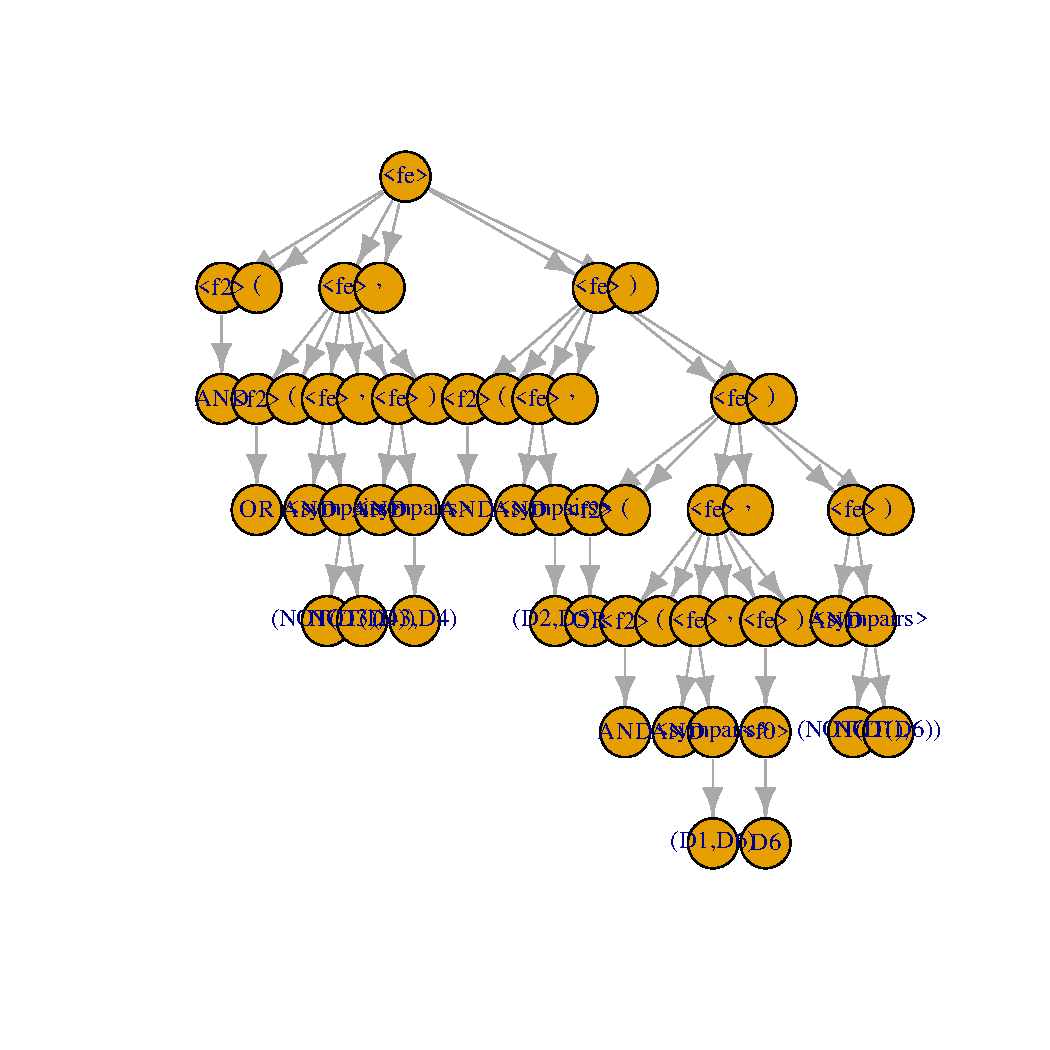
\includegraphics[width=0.5\textwidth, angle=0]
{ExpEDerivationTreeFigure004.pdf}
 \end{center}
 \label{report/ExpEDerivationTreeFigure004.pdf}  
 \end{frame}

% report/ExpEmain085.tex
% ExpE
% Figure: Plot of last xegaRun for Treatment BoolT4sgp6k of Experiment ExpE
% Thu May  8 17:40:54 2025
 \begin{frame}
 \frametitle{ Plot of last xegaRun for Treatment BoolT4sgp6k of Experiment ExpE }
 \begin{center}
\includegraphics[width=0.5\textwidth, angle=-90]
{ExpEPlotPopStatsFigure004.eps}
 \end{center}
 \label{report/ExpEPlotPopStatsFigure004.eps}  
 \end{frame}

% report/ExpEmain086.tex
\miniframesoff
\subsection{Treatment BoolT5sgp2k}
% report/ExpEmain087.tex
% ExpE
% Table:  Parameters of treatment: BoolT5sgp2k 

% Thu May  8 17:40:54 2025
 \begin{frame}
 \fontsize{8pt}{9pt}\selectfont
 \frametitle{  Parameters of treatment: BoolT5sgp2k 
 }
% latex table generated in R 4.4.3 by xtable 1.8-4 package
% Wed May 14 17:33:41 2025
\begin{table}[ht]
\centering
\begin{tabular}{rr}
  \hline
 & Parameter Values \\ 
  \hline
tRNG & L'Ecuyer-CMRG Inversion Rejection \\ 
  tReplay & 0 \\ 
  experimentName & EE \\ 
  treatmentName & BoolT5sgp2k \\ 
  trials & 20 \\ 
  everyK & 10 \\ 
  outpath & data \\ 
  batchPath & . \\ 
  tVerbose & 1 \\ 
   \hline
\end{tabular}
\caption{ Parameters of treatment: BoolT5sgp2k 
} 
\end{table}

 \label{ExpEtParmTable020.tex}  
 \end{frame}

 % Label:  \label{ExpEtParmTable020.tex}  
% report/ExpEmain088.tex
% ExpE
% Table:  Parameters of treatment BoolT5sgp2k passed to xegaRun

% Thu May  8 17:40:54 2025
 \begin{frame}
 \fontsize{8pt}{9pt}\selectfont
 \frametitle{  Parameters of treatment BoolT5sgp2k passed to xegaRun
 }
% latex table generated in R 4.4.3 by xtable 1.8-4 package
% Wed May 14 17:33:41 2025
\begin{table}[ht]
\centering
\begin{tabular}{rr}
  \hline
 & Parameter Values \\ 
  \hline
penv & 2-Symmetry Problem \\ 
  grammar & /home/dj2333/dev/cran/kSymmetry/BNF/AndOrNotTuned5.txt \\ 
  replay & 0 \\ 
  algorithm & sgp \\ 
  maxdepth & 7 \\ 
  max & FALSE \\ 
  worstFitness & -4 \\ 
  popsize & 200 \\ 
  generations & 500 \\ 
  crossrate & 0.2 \\ 
  mutrate & 0.4 \\ 
  ivmutrate & Const \\ 
  mutrate2 & 0.8 \\ 
  ivcrossrate & Const \\ 
  crossrate2 & 0.4 \\ 
   \hline
\end{tabular}
\caption{ Parameters of treatment BoolT5sgp2k passed to xegaRun
 (Part 1)} 
\end{table}

 \label{ExpEtParmTable021.tex}  
 \end{frame}

 % Label:  \label{ExpEtParmTable021.tex}  
% report/ExpEmain089.tex
% ExpE
% Table:  Parameters of treatment BoolT5sgp2k passed to xegaRun

% Thu May  8 17:40:54 2025
 \begin{frame}
 \fontsize{8pt}{9pt}\selectfont
 \frametitle{  Parameters of treatment BoolT5sgp2k passed to xegaRun
 }
% latex table generated in R 4.4.3 by xtable 1.8-4 package
% Thu May  8 17:40:54 2025
\begin{table}[ht]
\centering
\begin{tabular}{rr}
  \hline
 & Parameter Values \\ 
  \hline
scalefactor & Uniform \\ 
  genemap & Bin2Dec \\ 
  initgene & InitGene \\ 
  selection & SUS \\ 
  mateselection & SUS \\ 
  replication & Kid2 \\ 
  crossover & Cross2Gene \\ 
  mutation & MutateGene \\ 
  accept & All \\ 
  reportEvalErrors & TRUE \\ 
  codons & 80 \\ 
  codonPrecision & LCM \\ 
  terminationEps & -0.1 \\ 
  terminationCondition & AbsoluteError \\ 
  evalmethod & Deterministic \\ 
   \hline
\end{tabular}
\caption{ Parameters of treatment BoolT5sgp2k passed to xegaRun
 (Part 2)} 
\end{table}

 \label{ExpEtParmTable022.tex}  
 \end{frame}

 % Label:  \label{ExpEtParmTable022.tex}  
% report/ExpEmain090.tex
% ExpE
% Table:  Parameters of treatment BoolT5sgp2k passed to xegaRun

% Thu May  8 17:40:54 2025
 \begin{frame}
 \fontsize{8pt}{9pt}\selectfont
 \frametitle{  Parameters of treatment BoolT5sgp2k passed to xegaRun
 }
% latex table generated in R 4.4.3 by xtable 1.8-4 package
% Thu May  8 17:40:54 2025
\begin{table}[ht]
\centering
\begin{tabular}{rr}
  \hline
 & Parameter Values \\ 
  \hline
executionModel & MultiCore \\ 
  verbose & 1 \\ 
  batch & FALSE \\ 
  semantics & byValue \\ 
  path & . \\ 
   \hline
\end{tabular}
\caption{ Parameters of treatment BoolT5sgp2k passed to xegaRun
 (Part 3)} 
\end{table}

 \label{ExpEtParmTable023.tex}  
 \end{frame}

 % Label:  \label{ExpEtParmTable023.tex}  
% report/ExpEmain091.tex
% ExpE
% Table: The Production Table of Treatment BoolT5sgp2k of Experiment ExpE
% Thu May  8 17:40:54 2025
 \begin{frame}
 \fontsize{8pt}{9pt}\selectfont
 \frametitle{ The Production Table of Treatment BoolT5sgp2k of Experiment ExpE }
% latex table generated in R 4.4.3 by xtable 1.8-4 package
% Wed May 14 17:33:41 2025
\begin{table}[ht]
\centering
\begin{tabular}{rrr}
  \hline
 & LHS & RHS \\ 
  \hline
1 & $<$fe$>$ & $<$f0$>$ \\ 
  2 & $<$fe$>$ & $<$f1$>$($<$fe$>$) \\ 
  3 & $<$fe$>$ & $<$f2$>$($<$fe$>$,$<$fe$>$) \\ 
  4 & $<$f0$>$ & D1 \\ 
  5 & $<$f0$>$ & D2 \\ 
  6 & $<$fe$>$ & sPair$<$sympairs$>$ \\ 
  7 & $<$sympairs$>$ & (D1,D2) \\ 
  8 & $<$sympairs$>$ & (NOT(D1),NOT(D2)) \\ 
  9 & $<$f1$>$ & NOT \\ 
  10 & $<$f2$>$ & OR \\ 
  11 & $<$f2$>$ & AND \\ 
   \hline
\end{tabular}
\caption{The Production Table of Treatment BoolT5sgp2k of Experiment ExpE} 
\end{table}

 \label{ExpEGrammarTable008.tex}  
 \end{frame}

 % Label:  \label{ExpEGrammarTable008.tex}  
% report/ExpEmain092.tex
% ExpE
% Table: Treatment: BoolT5sgp2k
% Thu May  8 17:40:54 2025
 \begin{frame}
 \fontsize{8pt}{9pt}\selectfont
 \frametitle{ Treatment: BoolT5sgp2k }
% latex table generated in R 4.4.3 by xtable 1.8-4 package
% Wed May 14 17:33:41 2025
\begin{table}[ht]
\centering
\begin{tabular}{rrrrrrrr}
  \hline
 & Treatment & Trials & Variable & min & mean & sd & max \\ 
  \hline
24 & BoolT5sgp2k &  80 & Evaluations & 200.00 & 200.00 & 0.00 & 200.00 \\ 
  21 & BoolT5sgp2k &  80 & Fitness & 0.00 & 0.00 & 0.00 & 0.00 \\ 
  23 & BoolT5sgp2k &  80 & Generations & 1.00 & 1.00 & 0.00 & 1.00 \\ 
  22 & BoolT5sgp2k &  80 & Seconds & 0.17 & 0.22 & 0.02 & 0.29 \\ 
   \hline
\end{tabular}
\caption{Treatment: BoolT5sgp2k} 
\end{table}

 \label{ExpEStatsTable008.tex}  
 \end{frame}

 % Label:  \label{ExpEStatsTable008.tex}  
% report/ExpEmain093.tex
% ExpE
% Table: The Solution Table of Treatment BoolT5sgp2k of Experiment ExpE. Fit: 0. Unique Shortest Solutions: 13.
% Thu May  8 17:40:54 2025
 \begin{frame}
 \fontsize{8pt}{9pt}\selectfont
 \frametitle{ The Solution Table of Treatment BoolT5sgp2k of Experiment ExpE. Fit: 0. Unique Shortest Solutions: 13. }
% latex table generated in R 4.4.3 by xtable 1.8-4 package
% Wed May 14 17:33:42 2025
\begin{table}[ht]
\centering
\begin{tabular}{rp{9cm}}
  \hline
 & Solution \\ 
  \hline
1 & sPair(D1, D2) \\ 
   \hline
\end{tabular}
\caption{The Solution Table of Treatment BoolT5sgp2k of Experiment ExpE. Fit: 0. Unique Shortest Solutions: 13.} 
\end{table}

 \label{ExpESolutionTable005.tex}  
 \end{frame}

 % Label:  \label{ExpESolutionTable005.tex}  
% report/ExpEmain094.tex
% ExpE
% Figure: The Derivation Tree of a Solution of Treatment BoolT5sgp2k of Experiment ExpE
% Thu May  8 17:40:54 2025
 \begin{frame}
 \frametitle{ The Derivation Tree of a Solution of Treatment BoolT5sgp2k of Experiment ExpE }
 \begin{center}
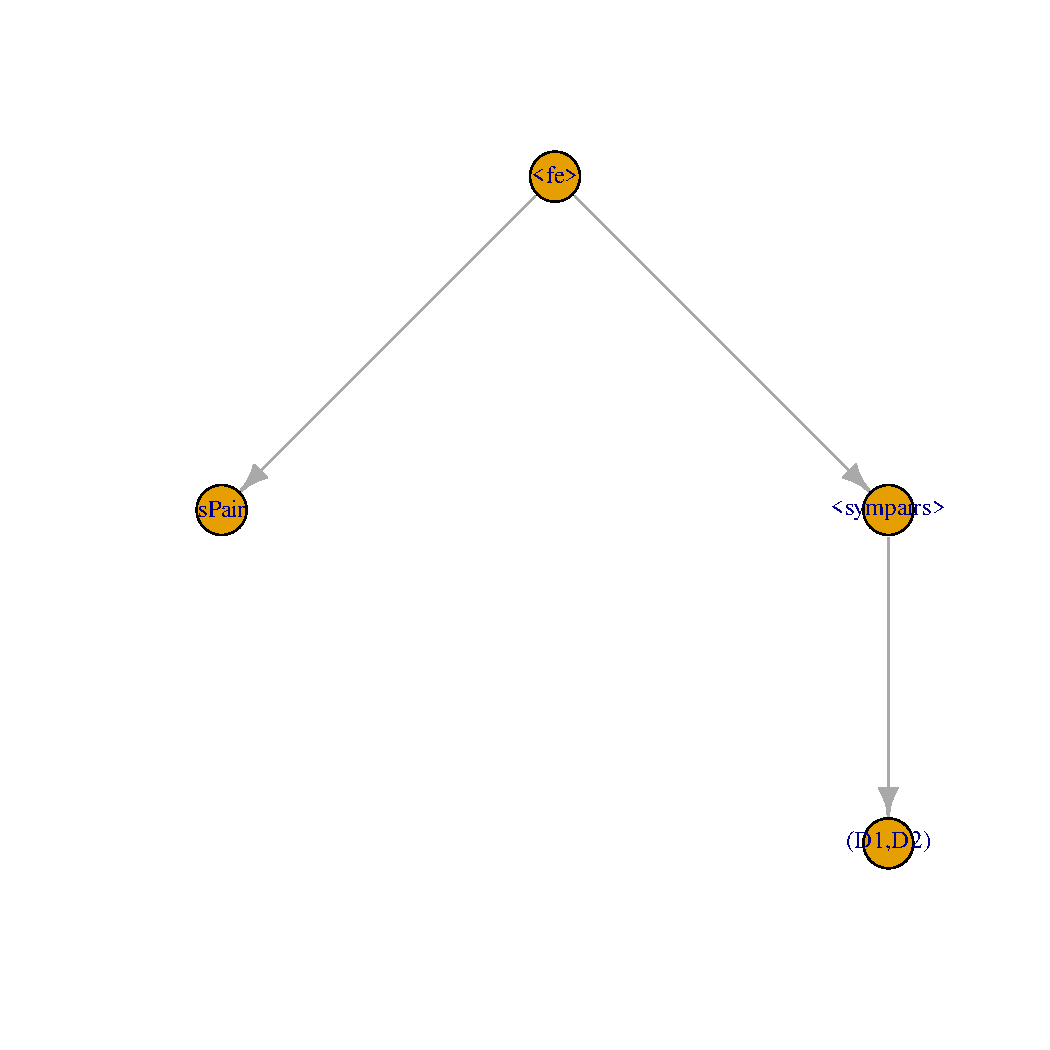
\includegraphics[width=0.5\textwidth, angle=0]
{ExpEDerivationTreeFigure005.pdf}
 \end{center}
 \label{report/ExpEDerivationTreeFigure005.pdf}  
 \end{frame}

% report/ExpEmain095.tex
% ExpE
% Figure: Plot of last xegaRun for Treatment BoolT5sgp2k of Experiment ExpE
% Thu May  8 17:40:54 2025
 \begin{frame}
 \frametitle{ Plot of last xegaRun for Treatment BoolT5sgp2k of Experiment ExpE }
 \begin{center}
\includegraphics[width=0.5\textwidth, angle=-90]
{ExpEPlotPopStatsFigure005.eps}
 \end{center}
 \label{report/ExpEPlotPopStatsFigure005.eps}  
 \end{frame}

% report/ExpEmain096.tex
\miniframesoff
\subsection{Treatment BoolT5sgp3k}
% report/ExpEmain097.tex
% ExpE
% Table:  Parameters of treatment: BoolT5sgp3k 

% Thu May  8 17:40:54 2025
 \begin{frame}
 \fontsize{8pt}{9pt}\selectfont
 \frametitle{  Parameters of treatment: BoolT5sgp3k 
 }
% latex table generated in R 4.4.3 by xtable 1.8-4 package
% Wed May 14 17:33:42 2025
\begin{table}[ht]
\centering
\begin{tabular}{rr}
  \hline
 & Parameter Values \\ 
  \hline
tRNG & L'Ecuyer-CMRG Inversion Rejection \\ 
  tReplay & 0 \\ 
  experimentName & EE \\ 
  treatmentName & BoolT5sgp3k \\ 
  trials & 20 \\ 
  everyK & 10 \\ 
  outpath & data \\ 
  batchPath & . \\ 
  tVerbose & 1 \\ 
   \hline
\end{tabular}
\caption{ Parameters of treatment: BoolT5sgp3k 
} 
\end{table}

 \label{ExpEtParmTable024.tex}  
 \end{frame}

 % Label:  \label{ExpEtParmTable024.tex}  
% report/ExpEmain098.tex
% ExpE
% Table:  Parameters of treatment BoolT5sgp3k passed to xegaRun

% Thu May  8 17:40:54 2025
 \begin{frame}
 \fontsize{8pt}{9pt}\selectfont
 \frametitle{  Parameters of treatment BoolT5sgp3k passed to xegaRun
 }
% latex table generated in R 4.4.3 by xtable 1.8-4 package
% Thu May  8 17:40:54 2025
\begin{table}[ht]
\centering
\begin{tabular}{rr}
  \hline
 & Parameter Values \\ 
  \hline
penv & 3-Symmetry Problem \\ 
  grammar & /home/dj2333/dev/cran/kSymmetry/BNF/AndOrNotTuned5.txt \\ 
  replay & 0 \\ 
  algorithm & sgp \\ 
  maxdepth & 7 \\ 
  max & FALSE \\ 
  worstFitness & -8 \\ 
  popsize & 200 \\ 
  generations & 500 \\ 
  crossrate & 0.2 \\ 
  mutrate & 0.4 \\ 
  ivmutrate & Const \\ 
  mutrate2 & 0.8 \\ 
  ivcrossrate & Const \\ 
  crossrate2 & 0.4 \\ 
   \hline
\end{tabular}
\caption{ Parameters of treatment BoolT5sgp3k passed to xegaRun
 (Part 1)} 
\end{table}

 \label{ExpEtParmTable025.tex}  
 \end{frame}

 % Label:  \label{ExpEtParmTable025.tex}  
% report/ExpEmain099.tex
% ExpE
% Table:  Parameters of treatment BoolT5sgp3k passed to xegaRun

% Thu May  8 17:40:54 2025
 \begin{frame}
 \fontsize{8pt}{9pt}\selectfont
 \frametitle{  Parameters of treatment BoolT5sgp3k passed to xegaRun
 }
% latex table generated in R 4.4.3 by xtable 1.8-4 package
% Wed May 14 17:33:42 2025
\begin{table}[ht]
\centering
\begin{tabular}{rr}
  \hline
 & Parameter Values \\ 
  \hline
scalefactor & Uniform \\ 
  genemap & Bin2Dec \\ 
  initgene & InitGene \\ 
  selection & SUS \\ 
  mateselection & SUS \\ 
  replication & Kid2 \\ 
  crossover & Cross2Gene \\ 
  mutation & MutateGene \\ 
  accept & All \\ 
  reportEvalErrors & TRUE \\ 
  codons & 120 \\ 
  codonPrecision & LCM \\ 
  terminationEps & -0.1 \\ 
  terminationCondition & AbsoluteError \\ 
  evalmethod & Deterministic \\ 
   \hline
\end{tabular}
\caption{ Parameters of treatment BoolT5sgp3k passed to xegaRun
 (Part 2)} 
\end{table}

 \label{ExpEtParmTable026.tex}  
 \end{frame}

 % Label:  \label{ExpEtParmTable026.tex}  
% report/ExpEmain100.tex
% ExpE
% Table:  Parameters of treatment BoolT5sgp3k passed to xegaRun

% Thu May  8 17:40:54 2025
 \begin{frame}
 \fontsize{8pt}{9pt}\selectfont
 \frametitle{  Parameters of treatment BoolT5sgp3k passed to xegaRun
 }
% latex table generated in R 4.4.3 by xtable 1.8-4 package
% Thu May  8 17:40:54 2025
\begin{table}[ht]
\centering
\begin{tabular}{rr}
  \hline
 & Parameter Values \\ 
  \hline
executionModel & MultiCore \\ 
  verbose & 1 \\ 
  batch & FALSE \\ 
  semantics & byValue \\ 
  path & . \\ 
   \hline
\end{tabular}
\caption{ Parameters of treatment BoolT5sgp3k passed to xegaRun
 (Part 3)} 
\end{table}

 \label{ExpEtParmTable027.tex}  
 \end{frame}

 % Label:  \label{ExpEtParmTable027.tex}  
% report/ExpEmain101.tex
% ExpE
% Table: The Production Table of Treatment BoolT5sgp3k of Experiment ExpE
% Thu May  8 17:40:54 2025
 \begin{frame}
 \fontsize{8pt}{9pt}\selectfont
 \frametitle{ The Production Table of Treatment BoolT5sgp3k of Experiment ExpE }
% latex table generated in R 4.4.3 by xtable 1.8-4 package
% Wed May 14 17:33:42 2025
\begin{table}[ht]
\centering
\begin{tabular}{rrr}
  \hline
 & LHS & RHS \\ 
  \hline
1 & $<$fe$>$ & $<$f0$>$ \\ 
  2 & $<$fe$>$ & $<$f1$>$($<$fe$>$) \\ 
  3 & $<$fe$>$ & $<$f2$>$($<$fe$>$,$<$fe$>$) \\ 
  4 & $<$f0$>$ & D1 \\ 
  5 & $<$f0$>$ & D2 \\ 
  6 & $<$f0$>$ & D3 \\ 
  7 & $<$fe$>$ & sPair$<$sympairs$>$ \\ 
  8 & $<$sympairs$>$ & (D1,D3) \\ 
  9 & $<$sympairs$>$ & (NOT(D1),NOT(D3)) \\ 
  10 & $<$f1$>$ & NOT \\ 
  11 & $<$f2$>$ & OR \\ 
  12 & $<$f2$>$ & AND \\ 
   \hline
\end{tabular}
\caption{The Production Table of Treatment BoolT5sgp3k of Experiment ExpE} 
\end{table}

 \label{ExpEGrammarTable009.tex}  
 \end{frame}

 % Label:  \label{ExpEGrammarTable009.tex}  
% report/ExpEmain102.tex
% ExpE
% Table: Treatment: BoolT5sgp3k
% Thu May  8 17:40:55 2025
 \begin{frame}
 \fontsize{8pt}{9pt}\selectfont
 \frametitle{ Treatment: BoolT5sgp3k }
% latex table generated in R 4.4.3 by xtable 1.8-4 package
% Wed May 14 17:33:42 2025
\begin{table}[ht]
\centering
\begin{tabular}{rrrrrrrr}
  \hline
 & Treatment & Trials & Variable & min & mean & sd & max \\ 
  \hline
28 & BoolT5sgp3k &  80 & Evaluations & 200.00 & 200.00 & 0.00 & 200.00 \\ 
  25 & BoolT5sgp3k &  80 & Fitness & 0.00 & 0.00 & 0.00 & 0.00 \\ 
  27 & BoolT5sgp3k &  80 & Generations & 1.00 & 1.00 & 0.00 & 1.00 \\ 
  26 & BoolT5sgp3k &  80 & Seconds & 0.20 & 0.25 & 0.03 & 0.35 \\ 
   \hline
\end{tabular}
\caption{Treatment: BoolT5sgp3k} 
\end{table}

 \label{ExpEStatsTable009.tex}  
 \end{frame}

 % Label:  \label{ExpEStatsTable009.tex}  
% report/ExpEmain103.tex
% ExpE
% Table: The Solution Table of Treatment BoolT5sgp3k of Experiment ExpE. Fit: 0. Unique Shortest Solutions: 11.
% Thu May  8 17:40:55 2025
 \begin{frame}
 \fontsize{8pt}{9pt}\selectfont
 \frametitle{ The Solution Table of Treatment BoolT5sgp3k of Experiment ExpE. Fit: 0. Unique Shortest Solutions: 11. }
% latex table generated in R 4.4.3 by xtable 1.8-4 package
% Wed May 14 17:33:42 2025
\begin{table}[ht]
\centering
\begin{tabular}{rp{9cm}}
  \hline
 & Solution \\ 
  \hline
1 & sPair(D1, D3) \\ 
   \hline
\end{tabular}
\caption{The Solution Table of Treatment BoolT5sgp3k of Experiment ExpE. Fit: 0. Unique Shortest Solutions: 11.} 
\end{table}

 \label{ExpESolutionTable006.tex}  
 \end{frame}

 % Label:  \label{ExpESolutionTable006.tex}  
% report/ExpEmain104.tex
% ExpE
% Figure: The Derivation Tree of a Solution of Treatment BoolT5sgp3k of Experiment ExpE
% Thu May  8 17:40:55 2025
 \begin{frame}
 \frametitle{ The Derivation Tree of a Solution of Treatment BoolT5sgp3k of Experiment ExpE }
 \begin{center}
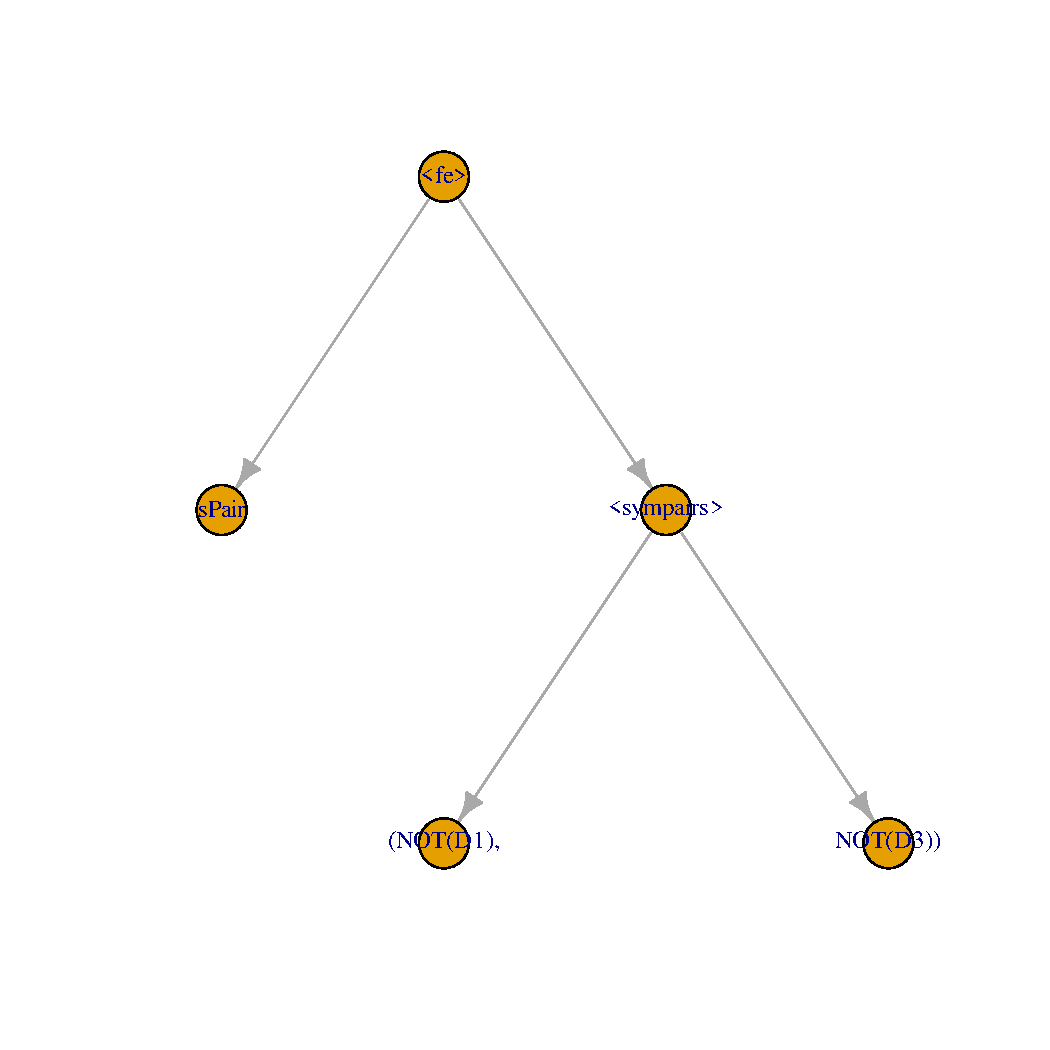
\includegraphics[width=0.5\textwidth, angle=0]
{ExpEDerivationTreeFigure006.pdf}
 \end{center}
 \label{report/ExpEDerivationTreeFigure006.pdf}  
 \end{frame}

% report/ExpEmain105.tex
% ExpE
% Figure: Plot of last xegaRun for Treatment BoolT5sgp3k of Experiment ExpE
% Thu May  8 17:40:55 2025
 \begin{frame}
 \frametitle{ Plot of last xegaRun for Treatment BoolT5sgp3k of Experiment ExpE }
 \begin{center}
\includegraphics[width=0.5\textwidth, angle=-90]
{ExpEPlotPopStatsFigure006.eps}
 \end{center}
 \label{report/ExpEPlotPopStatsFigure006.eps}  
 \end{frame}

% report/ExpEmain106.tex
\miniframesoff
\subsection{Treatment BoolT5sgp4k}
% report/ExpEmain107.tex
% ExpE
% Table:  Parameters of treatment: BoolT5sgp4k 

% Thu May  8 17:40:55 2025
 \begin{frame}
 \fontsize{8pt}{9pt}\selectfont
 \frametitle{  Parameters of treatment: BoolT5sgp4k 
 }
% latex table generated in R 4.4.3 by xtable 1.8-4 package
% Wed May 14 17:33:42 2025
\begin{table}[ht]
\centering
\begin{tabular}{rr}
  \hline
 & Parameter Values \\ 
  \hline
tRNG & L'Ecuyer-CMRG Inversion Rejection \\ 
  tReplay & 0 \\ 
  experimentName & EE \\ 
  treatmentName & BoolT5sgp4k \\ 
  trials & 20 \\ 
  everyK & 10 \\ 
  outpath & data \\ 
  batchPath & . \\ 
  tVerbose & 1 \\ 
   \hline
\end{tabular}
\caption{ Parameters of treatment: BoolT5sgp4k 
} 
\end{table}

 \label{ExpEtParmTable028.tex}  
 \end{frame}

 % Label:  \label{ExpEtParmTable028.tex}  
% report/ExpEmain108.tex
% ExpE
% Table:  Parameters of treatment BoolT5sgp4k passed to xegaRun

% Thu May  8 17:40:55 2025
 \begin{frame}
 \fontsize{8pt}{9pt}\selectfont
 \frametitle{  Parameters of treatment BoolT5sgp4k passed to xegaRun
 }
% latex table generated in R 4.4.3 by xtable 1.8-4 package
% Wed May 14 17:33:42 2025
\begin{table}[ht]
\centering
\begin{tabular}{rr}
  \hline
 & Parameter Values \\ 
  \hline
penv & 4-Symmetry Problem \\ 
  grammar & /home/dj2333/dev/cran/kSymmetry/BNF/AndOrNotTuned5.txt \\ 
  replay & 0 \\ 
  algorithm & sgp \\ 
  maxdepth & 7 \\ 
  max & FALSE \\ 
  worstFitness & -16 \\ 
  popsize & 200 \\ 
  generations & 500 \\ 
  crossrate & 0.2 \\ 
  mutrate & 0.4 \\ 
  ivmutrate & Const \\ 
  mutrate2 & 0.8 \\ 
  ivcrossrate & Const \\ 
  crossrate2 & 0.4 \\ 
   \hline
\end{tabular}
\caption{ Parameters of treatment BoolT5sgp4k passed to xegaRun
 (Part 1)} 
\end{table}

 \label{ExpEtParmTable029.tex}  
 \end{frame}

 % Label:  \label{ExpEtParmTable029.tex}  
% report/ExpEmain109.tex
% ExpE
% Table:  Parameters of treatment BoolT5sgp4k passed to xegaRun

% Thu May  8 17:40:55 2025
 \begin{frame}
 \fontsize{8pt}{9pt}\selectfont
 \frametitle{  Parameters of treatment BoolT5sgp4k passed to xegaRun
 }
% latex table generated in R 4.4.3 by xtable 1.8-4 package
% Thu May  8 17:40:55 2025
\begin{table}[ht]
\centering
\begin{tabular}{rr}
  \hline
 & Parameter Values \\ 
  \hline
scalefactor & Uniform \\ 
  genemap & Bin2Dec \\ 
  initgene & InitGene \\ 
  selection & SUS \\ 
  mateselection & SUS \\ 
  replication & Kid2 \\ 
  crossover & Cross2Gene \\ 
  mutation & MutateGene \\ 
  accept & All \\ 
  reportEvalErrors & TRUE \\ 
  codons & 160 \\ 
  codonPrecision & LCM \\ 
  terminationEps & -0.1 \\ 
  terminationCondition & AbsoluteError \\ 
  evalmethod & Deterministic \\ 
   \hline
\end{tabular}
\caption{ Parameters of treatment BoolT5sgp4k passed to xegaRun
 (Part 2)} 
\end{table}

 \label{ExpEtParmTable030.tex}  
 \end{frame}

 % Label:  \label{ExpEtParmTable030.tex}  
% report/ExpEmain110.tex
% ExpE
% Table:  Parameters of treatment BoolT5sgp4k passed to xegaRun

% Thu May  8 17:40:55 2025
 \begin{frame}
 \fontsize{8pt}{9pt}\selectfont
 \frametitle{  Parameters of treatment BoolT5sgp4k passed to xegaRun
 }
% latex table generated in R 4.4.3 by xtable 1.8-4 package
% Wed May 14 17:33:42 2025
\begin{table}[ht]
\centering
\begin{tabular}{rr}
  \hline
 & Parameter Values \\ 
  \hline
executionModel & MultiCore \\ 
  verbose & 1 \\ 
  batch & FALSE \\ 
  semantics & byValue \\ 
  path & . \\ 
   \hline
\end{tabular}
\caption{ Parameters of treatment BoolT5sgp4k passed to xegaRun
 (Part 3)} 
\end{table}

 \label{ExpEtParmTable031.tex}  
 \end{frame}

 % Label:  \label{ExpEtParmTable031.tex}  
% report/ExpEmain111.tex
% ExpE
% Table: The Production Table of Treatment BoolT5sgp4k of Experiment ExpE
% Thu May  8 17:40:55 2025
 \begin{frame}
 \fontsize{8pt}{9pt}\selectfont
 \frametitle{ The Production Table of Treatment BoolT5sgp4k of Experiment ExpE }
% latex table generated in R 4.4.3 by xtable 1.8-4 package
% Wed May 14 17:33:42 2025
\begin{table}[ht]
\centering
\begin{tabular}{rrr}
  \hline
 & LHS & RHS \\ 
  \hline
1 & $<$fe$>$ & $<$f0$>$ \\ 
  2 & $<$fe$>$ & $<$f1$>$($<$fe$>$) \\ 
  3 & $<$fe$>$ & $<$f2$>$($<$fe$>$,$<$fe$>$) \\ 
  4 & $<$f0$>$ & D1 \\ 
  5 & $<$f0$>$ & D2 \\ 
  6 & $<$f0$>$ & D3 \\ 
  7 & $<$f0$>$ & D4 \\ 
  8 & $<$fe$>$ & sPair$<$sympairs$>$ \\ 
  9 & $<$sympairs$>$ & (D1,D4) \\ 
  10 & $<$sympairs$>$ & (NOT(D1),NOT(D4)) \\ 
  11 & $<$sympairs$>$ & (D2,D3) \\ 
  12 & $<$sympairs$>$ & (NOT(D2),NOT(D3)) \\ 
  13 & $<$f1$>$ & NOT \\ 
  14 & $<$f2$>$ & OR \\ 
  15 & $<$f2$>$ & AND \\ 
   \hline
\end{tabular}
\caption{The Production Table of Treatment BoolT5sgp4k of Experiment ExpE} 
\end{table}

 \label{ExpEGrammarTable010.tex}  
 \end{frame}

 % Label:  \label{ExpEGrammarTable010.tex}  
% report/ExpEmain112.tex
% ExpE
% Table: Treatment: BoolT5sgp4k
% Thu May  8 17:40:55 2025
 \begin{frame}
 \fontsize{8pt}{9pt}\selectfont
 \frametitle{ Treatment: BoolT5sgp4k }
% latex table generated in R 4.4.3 by xtable 1.8-4 package
% Wed May 14 17:33:42 2025
\begin{table}[ht]
\centering
\begin{tabular}{rrrrrrrr}
  \hline
 & Treatment & Trials & Variable & min & mean & sd & max \\ 
  \hline
32 & BoolT5sgp4k &  80 & Evaluations & 200.00 & 245.00 & 110.12 & 800.00 \\ 
  29 & BoolT5sgp4k &  80 & Fitness & 0.00 & 0.00 & 0.00 & 0.00 \\ 
  31 & BoolT5sgp4k &  80 & Generations & 1.00 & 1.23 & 0.55 & 4.00 \\ 
  30 & BoolT5sgp4k &  80 & Seconds & 0.20 & 0.31 & 0.11 & 0.91 \\ 
   \hline
\end{tabular}
\caption{Treatment: BoolT5sgp4k} 
\end{table}

 \label{ExpEStatsTable010.tex}  
 \end{frame}

 % Label:  \label{ExpEStatsTable010.tex}  
% report/ExpEmain113.tex
% ExpE
% Table: The Solution Table of Treatment BoolT5sgp4k of Experiment ExpE. Fit: 0. Unique Shortest Solutions: 39.
% Thu May  8 17:40:55 2025
 \begin{frame}
 \fontsize{8pt}{9pt}\selectfont
 \frametitle{ The Solution Table of Treatment BoolT5sgp4k of Experiment ExpE. Fit: 0. Unique Shortest Solutions: 39. }
% latex table generated in R 4.4.3 by xtable 1.8-4 package
% Wed May 14 17:33:42 2025
\begin{table}[ht]
\centering
\begin{tabular}{rp{9cm}}
  \hline
 & Solution \\ 
  \hline
1 & AND(sPair(D2, D3), sPair(D1, D4)) \\ 
   \hline
\end{tabular}
\caption{The Solution Table of Treatment BoolT5sgp4k of Experiment ExpE. Fit: 0. Unique Shortest Solutions: 39.} 
\end{table}

 \label{ExpESolutionTable007.tex}  
 \end{frame}

 % Label:  \label{ExpESolutionTable007.tex}  
% report/ExpEmain114.tex
% ExpE
% Figure: The Derivation Tree of a Solution of Treatment BoolT5sgp4k of Experiment ExpE
% Thu May  8 17:40:55 2025
 \begin{frame}
 \frametitle{ The Derivation Tree of a Solution of Treatment BoolT5sgp4k of Experiment ExpE }
 \begin{center}
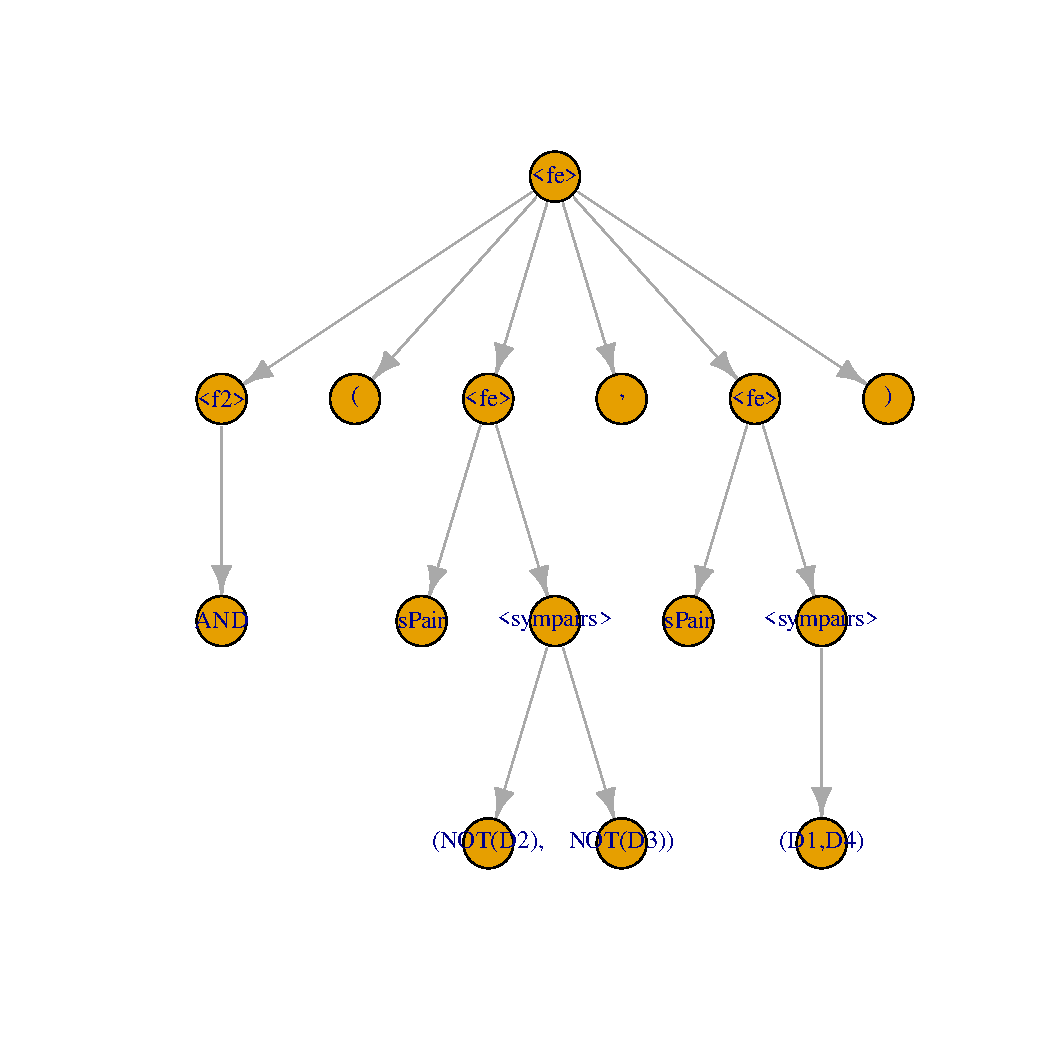
\includegraphics[width=0.5\textwidth, angle=0]
{ExpEDerivationTreeFigure007.pdf}
 \end{center}
 \label{report/ExpEDerivationTreeFigure007.pdf}  
 \end{frame}

% report/ExpEmain115.tex
% ExpE
% Figure: Plot of last xegaRun for Treatment BoolT5sgp4k of Experiment ExpE
% Thu May  8 17:40:55 2025
 \begin{frame}
 \frametitle{ Plot of last xegaRun for Treatment BoolT5sgp4k of Experiment ExpE }
 \begin{center}
\includegraphics[width=0.5\textwidth, angle=-90]
{ExpEPlotPopStatsFigure007.eps}
 \end{center}
 \label{report/ExpEPlotPopStatsFigure007.eps}  
 \end{frame}

% report/ExpEmain116.tex
\miniframesoff
\subsection{Treatment BoolT5sgp5k}
% report/ExpEmain117.tex
% ExpE
% Table:  Parameters of treatment: BoolT5sgp5k 

% Thu May  8 17:40:55 2025
 \begin{frame}
 \fontsize{8pt}{9pt}\selectfont
 \frametitle{  Parameters of treatment: BoolT5sgp5k 
 }
% latex table generated in R 4.4.3 by xtable 1.8-4 package
% Thu May  8 17:40:55 2025
\begin{table}[ht]
\centering
\begin{tabular}{rr}
  \hline
 & Parameter Values \\ 
  \hline
tRNG & L'Ecuyer-CMRG Inversion Rejection \\ 
  tReplay & 0 \\ 
  experimentName & EE \\ 
  treatmentName & BoolT5sgp5k \\ 
  trials & 20 \\ 
  everyK & 10 \\ 
  outpath & data \\ 
  batchPath & . \\ 
  tVerbose & 1 \\ 
   \hline
\end{tabular}
\caption{ Parameters of treatment: BoolT5sgp5k 
} 
\end{table}

 \label{ExpEtParmTable032.tex}  
 \end{frame}

 % Label:  \label{ExpEtParmTable032.tex}  
% report/ExpEmain118.tex
% ExpE
% Table:  Parameters of treatment BoolT5sgp5k passed to xegaRun

% Thu May  8 17:40:55 2025
 \begin{frame}
 \fontsize{8pt}{9pt}\selectfont
 \frametitle{  Parameters of treatment BoolT5sgp5k passed to xegaRun
 }
% latex table generated in R 4.4.3 by xtable 1.8-4 package
% Wed May 14 17:33:42 2025
\begin{table}[ht]
\centering
\begin{tabular}{rr}
  \hline
 & Parameter Values \\ 
  \hline
penv & 5-Symmetry Problem \\ 
  grammar & /home/dj2333/dev/cran/kSymmetry/BNF/AndOrNotTuned5.txt \\ 
  replay & 0 \\ 
  algorithm & sgp \\ 
  maxdepth & 7 \\ 
  max & FALSE \\ 
  worstFitness & -32 \\ 
  popsize & 200 \\ 
  generations & 500 \\ 
  crossrate & 0.2 \\ 
  mutrate & 0.4 \\ 
  ivmutrate & Const \\ 
  mutrate2 & 0.8 \\ 
  ivcrossrate & Const \\ 
  crossrate2 & 0.4 \\ 
   \hline
\end{tabular}
\caption{ Parameters of treatment BoolT5sgp5k passed to xegaRun
 (Part 1)} 
\end{table}

 \label{ExpEtParmTable033.tex}  
 \end{frame}

 % Label:  \label{ExpEtParmTable033.tex}  
% report/ExpEmain119.tex
% ExpE
% Table:  Parameters of treatment BoolT5sgp5k passed to xegaRun

% Thu May  8 17:40:55 2025
 \begin{frame}
 \fontsize{8pt}{9pt}\selectfont
 \frametitle{  Parameters of treatment BoolT5sgp5k passed to xegaRun
 }
% latex table generated in R 4.4.3 by xtable 1.8-4 package
% Thu May  8 17:40:55 2025
\begin{table}[ht]
\centering
\begin{tabular}{rr}
  \hline
 & Parameter Values \\ 
  \hline
scalefactor & Uniform \\ 
  genemap & Bin2Dec \\ 
  initgene & InitGene \\ 
  selection & SUS \\ 
  mateselection & SUS \\ 
  replication & Kid2 \\ 
  crossover & Cross2Gene \\ 
  mutation & MutateGene \\ 
  accept & All \\ 
  reportEvalErrors & TRUE \\ 
  codons & 200 \\ 
  codonPrecision & LCM \\ 
  terminationEps & -0.1 \\ 
  terminationCondition & AbsoluteError \\ 
  evalmethod & Deterministic \\ 
   \hline
\end{tabular}
\caption{ Parameters of treatment BoolT5sgp5k passed to xegaRun
 (Part 2)} 
\end{table}

 \label{ExpEtParmTable034.tex}  
 \end{frame}

 % Label:  \label{ExpEtParmTable034.tex}  
% report/ExpEmain120.tex
% ExpE
% Table:  Parameters of treatment BoolT5sgp5k passed to xegaRun

% Thu May  8 17:40:55 2025
 \begin{frame}
 \fontsize{8pt}{9pt}\selectfont
 \frametitle{  Parameters of treatment BoolT5sgp5k passed to xegaRun
 }
% latex table generated in R 4.4.3 by xtable 1.8-4 package
% Wed May 14 17:33:42 2025
\begin{table}[ht]
\centering
\begin{tabular}{rr}
  \hline
 & Parameter Values \\ 
  \hline
executionModel & MultiCore \\ 
  verbose & 1 \\ 
  batch & FALSE \\ 
  semantics & byValue \\ 
  path & . \\ 
   \hline
\end{tabular}
\caption{ Parameters of treatment BoolT5sgp5k passed to xegaRun
 (Part 3)} 
\end{table}

 \label{ExpEtParmTable035.tex}  
 \end{frame}

 % Label:  \label{ExpEtParmTable035.tex}  
% report/ExpEmain121.tex
% ExpE
% Table: The Production Table of Treatment BoolT5sgp5k of Experiment ExpE
% Thu May  8 17:40:55 2025
 \begin{frame}
 \fontsize{8pt}{9pt}\selectfont
 \frametitle{ The Production Table of Treatment BoolT5sgp5k of Experiment ExpE }
% latex table generated in R 4.4.3 by xtable 1.8-4 package
% Wed May 14 17:33:42 2025
\begin{table}[ht]
\centering
\begin{tabular}{rrr}
  \hline
 & LHS & RHS \\ 
  \hline
1 & $<$fe$>$ & $<$f0$>$ \\ 
  2 & $<$fe$>$ & $<$f1$>$($<$fe$>$) \\ 
  3 & $<$fe$>$ & $<$f2$>$($<$fe$>$,$<$fe$>$) \\ 
  4 & $<$f0$>$ & D1 \\ 
  5 & $<$f0$>$ & D2 \\ 
  6 & $<$f0$>$ & D3 \\ 
  7 & $<$f0$>$ & D4 \\ 
  8 & $<$f0$>$ & D5 \\ 
  9 & $<$fe$>$ & sPair$<$sympairs$>$ \\ 
  10 & $<$sympairs$>$ & (D1,D5) \\ 
  11 & $<$sympairs$>$ & (NOT(D1),NOT(D5)) \\ 
  12 & $<$sympairs$>$ & (D2,D4) \\ 
  13 & $<$sympairs$>$ & (NOT(D2),NOT(D4)) \\ 
  14 & $<$f1$>$ & NOT \\ 
  15 & $<$f2$>$ & OR \\ 
   \hline
\end{tabular}
\caption{The Production Table of Treatment BoolT5sgp5k of Experiment ExpE (Part 1)} 
\end{table}

 \label{ExpEGrammarTable011.tex}  
 \end{frame}

 % Label:  \label{ExpEGrammarTable011.tex}  
% report/ExpEmain122.tex
% ExpE
% Table: The Production Table of Treatment BoolT5sgp5k of Experiment ExpE
% Thu May  8 17:40:55 2025
 \begin{frame}
 \fontsize{8pt}{9pt}\selectfont
 \frametitle{ The Production Table of Treatment BoolT5sgp5k of Experiment ExpE }
% latex table generated in R 4.4.3 by xtable 1.8-4 package
% Thu May  8 17:40:55 2025
\begin{table}[ht]
\centering
\begin{tabular}{rrr}
  \hline
 & LHS & RHS \\ 
  \hline
16 & $<$f2$>$ & AND \\ 
   \hline
\end{tabular}
\caption{The Production Table of Treatment BoolT5sgp5k of Experiment ExpE (Part 2)} 
\end{table}

 \label{ExpEGrammarTable012.tex}  
 \end{frame}

 % Label:  \label{ExpEGrammarTable012.tex}  
% report/ExpEmain123.tex
% ExpE
% Table: Treatment: BoolT5sgp5k
% Thu May  8 17:40:55 2025
 \begin{frame}
 \fontsize{8pt}{9pt}\selectfont
 \frametitle{ Treatment: BoolT5sgp5k }
% latex table generated in R 4.4.3 by xtable 1.8-4 package
% Wed May 14 17:33:42 2025
\begin{table}[ht]
\centering
\begin{tabular}{rrrrrrrr}
  \hline
 & Treatment & Trials & Variable & min & mean & sd & max \\ 
  \hline
36 & BoolT5sgp5k &  80 & Evaluations & 200.00 & 240.00 & 112.06 & 800.00 \\ 
  33 & BoolT5sgp5k &  80 & Fitness & 0.00 & 0.00 & 0.00 & 0.00 \\ 
  35 & BoolT5sgp5k &  80 & Generations & 1.00 & 1.20 & 0.56 & 4.00 \\ 
  34 & BoolT5sgp5k &  80 & Seconds & 0.25 & 0.34 & 0.09 & 0.74 \\ 
   \hline
\end{tabular}
\caption{Treatment: BoolT5sgp5k} 
\end{table}

 \label{ExpEStatsTable011.tex}  
 \end{frame}

 % Label:  \label{ExpEStatsTable011.tex}  
% report/ExpEmain124.tex
% ExpE
% Table: The Solution Table of Treatment BoolT5sgp5k of Experiment ExpE. Fit: 0. Unique Shortest Solutions: 33.
% Thu May  8 17:40:55 2025
 \begin{frame}
 \fontsize{8pt}{9pt}\selectfont
 \frametitle{ The Solution Table of Treatment BoolT5sgp5k of Experiment ExpE. Fit: 0. Unique Shortest Solutions: 33. }
% latex table generated in R 4.4.3 by xtable 1.8-4 package
% Wed May 14 17:33:42 2025
\begin{table}[ht]
\centering
\begin{tabular}{rp{9cm}}
  \hline
 & Solution \\ 
  \hline
1 & AND(sPair(D1, D5), sPair(D2, D4)) \\ 
   \hline
\end{tabular}
\caption{The Solution Table of Treatment BoolT5sgp5k of Experiment ExpE. Fit: 0. Unique Shortest Solutions: 33.} 
\end{table}

 \label{ExpESolutionTable008.tex}  
 \end{frame}

 % Label:  \label{ExpESolutionTable008.tex}  
% report/ExpEmain125.tex
% ExpE
% Figure: The Derivation Tree of a Solution of Treatment BoolT5sgp5k of Experiment ExpE
% Thu May  8 17:40:55 2025
 \begin{frame}
 \frametitle{ The Derivation Tree of a Solution of Treatment BoolT5sgp5k of Experiment ExpE }
 \begin{center}
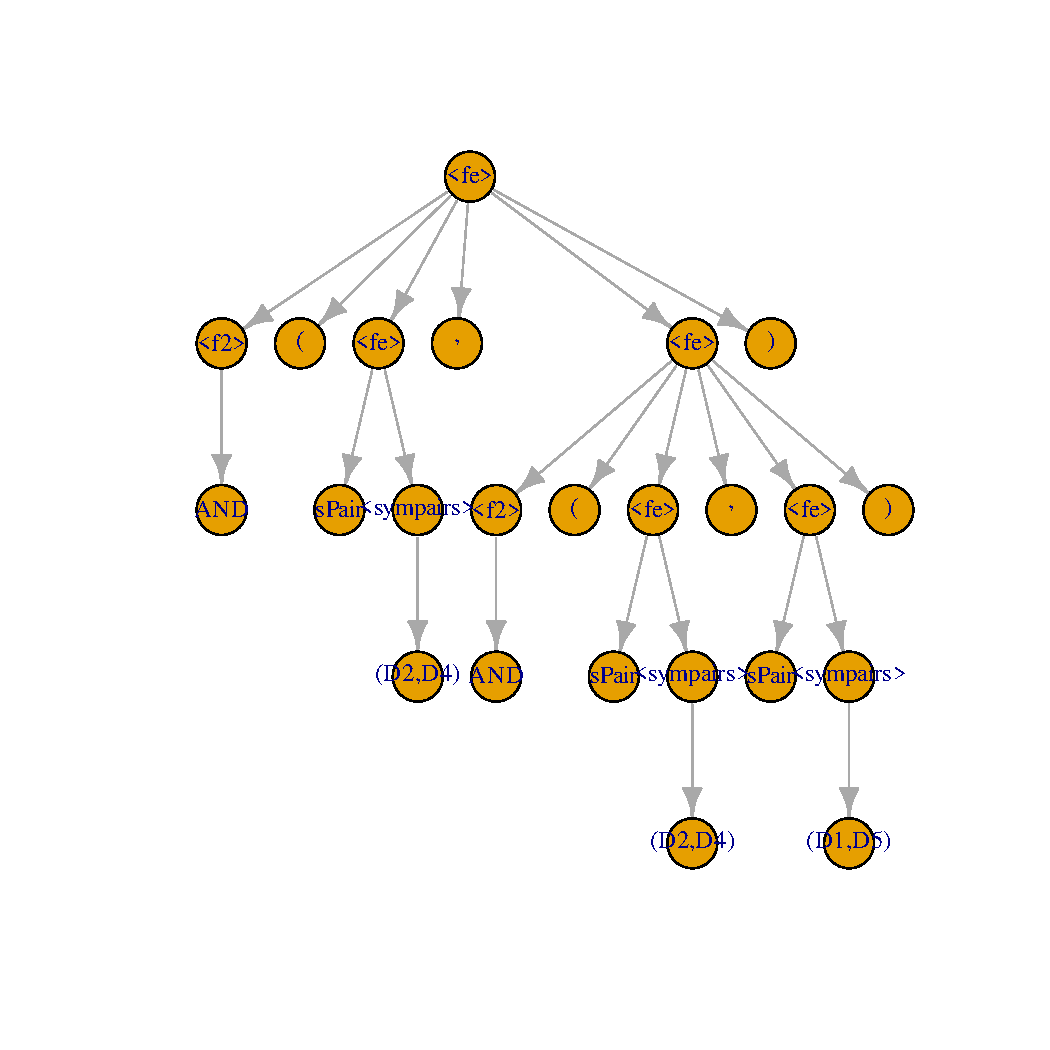
\includegraphics[width=0.5\textwidth, angle=0]
{ExpEDerivationTreeFigure008.pdf}
 \end{center}
 \label{report/ExpEDerivationTreeFigure008.pdf}  
 \end{frame}

% report/ExpEmain126.tex
% ExpE
% Figure: Plot of last xegaRun for Treatment BoolT5sgp5k of Experiment ExpE
% Thu May  8 17:40:55 2025
 \begin{frame}
 \frametitle{ Plot of last xegaRun for Treatment BoolT5sgp5k of Experiment ExpE }
 \begin{center}
\includegraphics[width=0.5\textwidth, angle=-90]
{ExpEPlotPopStatsFigure008.eps}
 \end{center}
 \label{report/ExpEPlotPopStatsFigure008.eps}  
 \end{frame}

% report/ExpEmain127.tex
\miniframesoff
\subsection{Treatment BoolT5sgp6k}
% report/ExpEmain128.tex
% ExpE
% Table:  Parameters of treatment: BoolT5sgp6k 

% Thu May  8 17:40:55 2025
 \begin{frame}
 \fontsize{8pt}{9pt}\selectfont
 \frametitle{  Parameters of treatment: BoolT5sgp6k 
 }
% latex table generated in R 4.4.3 by xtable 1.8-4 package
% Thu May  8 17:40:55 2025
\begin{table}[ht]
\centering
\begin{tabular}{rr}
  \hline
 & Parameter Values \\ 
  \hline
tRNG & L'Ecuyer-CMRG Inversion Rejection \\ 
  tReplay & 0 \\ 
  experimentName & EE \\ 
  treatmentName & BoolT5sgp6k \\ 
  trials & 20 \\ 
  everyK & 10 \\ 
  outpath & data \\ 
  batchPath & . \\ 
  tVerbose & 1 \\ 
   \hline
\end{tabular}
\caption{ Parameters of treatment: BoolT5sgp6k 
} 
\end{table}

 \label{ExpEtParmTable036.tex}  
 \end{frame}

 % Label:  \label{ExpEtParmTable036.tex}  
% report/ExpEmain129.tex
% ExpE
% Table:  Parameters of treatment BoolT5sgp6k passed to xegaRun

% Thu May  8 17:40:55 2025
 \begin{frame}
 \fontsize{8pt}{9pt}\selectfont
 \frametitle{  Parameters of treatment BoolT5sgp6k passed to xegaRun
 }
% latex table generated in R 4.4.3 by xtable 1.8-4 package
% Wed May 14 17:33:42 2025
\begin{table}[ht]
\centering
\begin{tabular}{rr}
  \hline
 & Parameter Values \\ 
  \hline
penv & 6-Symmetry Problem \\ 
  grammar & /home/dj2333/dev/cran/kSymmetry/BNF/AndOrNotTuned5.txt \\ 
  replay & 0 \\ 
  algorithm & sgp \\ 
  maxdepth & 7 \\ 
  max & FALSE \\ 
  worstFitness & -64 \\ 
  popsize & 200 \\ 
  generations & 500 \\ 
  crossrate & 0.2 \\ 
  mutrate & 0.4 \\ 
  ivmutrate & Const \\ 
  mutrate2 & 0.8 \\ 
  ivcrossrate & Const \\ 
  crossrate2 & 0.4 \\ 
   \hline
\end{tabular}
\caption{ Parameters of treatment BoolT5sgp6k passed to xegaRun
 (Part 1)} 
\end{table}

 \label{ExpEtParmTable037.tex}  
 \end{frame}

 % Label:  \label{ExpEtParmTable037.tex}  
% report/ExpEmain130.tex
% ExpE
% Table:  Parameters of treatment BoolT5sgp6k passed to xegaRun

% Thu May  8 17:40:55 2025
 \begin{frame}
 \fontsize{8pt}{9pt}\selectfont
 \frametitle{  Parameters of treatment BoolT5sgp6k passed to xegaRun
 }
% latex table generated in R 4.4.3 by xtable 1.8-4 package
% Wed May 14 17:33:42 2025
\begin{table}[ht]
\centering
\begin{tabular}{rr}
  \hline
 & Parameter Values \\ 
  \hline
scalefactor & Uniform \\ 
  genemap & Bin2Dec \\ 
  initgene & InitGene \\ 
  selection & SUS \\ 
  mateselection & SUS \\ 
  replication & Kid2 \\ 
  crossover & Cross2Gene \\ 
  mutation & MutateGene \\ 
  accept & All \\ 
  reportEvalErrors & TRUE \\ 
  codons & 240 \\ 
  codonPrecision & LCM \\ 
  terminationEps & -0.1 \\ 
  terminationCondition & AbsoluteError \\ 
  evalmethod & Deterministic \\ 
   \hline
\end{tabular}
\caption{ Parameters of treatment BoolT5sgp6k passed to xegaRun
 (Part 2)} 
\end{table}

 \label{ExpEtParmTable038.tex}  
 \end{frame}

 % Label:  \label{ExpEtParmTable038.tex}  
% report/ExpEmain131.tex
% ExpE
% Table:  Parameters of treatment BoolT5sgp6k passed to xegaRun

% Thu May  8 17:40:55 2025
 \begin{frame}
 \fontsize{8pt}{9pt}\selectfont
 \frametitle{  Parameters of treatment BoolT5sgp6k passed to xegaRun
 }
% latex table generated in R 4.4.3 by xtable 1.8-4 package
% Wed May 14 17:33:42 2025
\begin{table}[ht]
\centering
\begin{tabular}{rr}
  \hline
 & Parameter Values \\ 
  \hline
executionModel & MultiCore \\ 
  verbose & 1 \\ 
  batch & FALSE \\ 
  semantics & byValue \\ 
  path & . \\ 
   \hline
\end{tabular}
\caption{ Parameters of treatment BoolT5sgp6k passed to xegaRun
 (Part 3)} 
\end{table}

 \label{ExpEtParmTable039.tex}  
 \end{frame}

 % Label:  \label{ExpEtParmTable039.tex}  
% report/ExpEmain132.tex
% ExpE
% Table: The Production Table of Treatment BoolT5sgp6k of Experiment ExpE
% Thu May  8 17:40:55 2025
 \begin{frame}
 \fontsize{8pt}{9pt}\selectfont
 \frametitle{ The Production Table of Treatment BoolT5sgp6k of Experiment ExpE }
% latex table generated in R 4.4.3 by xtable 1.8-4 package
% Thu May  8 17:40:55 2025
\begin{table}[ht]
\centering
\begin{tabular}{rrr}
  \hline
 & LHS & RHS \\ 
  \hline
1 & $<$fe$>$ & $<$f0$>$ \\ 
  2 & $<$fe$>$ & $<$f1$>$($<$fe$>$) \\ 
  3 & $<$fe$>$ & $<$f2$>$($<$fe$>$,$<$fe$>$) \\ 
  4 & $<$f0$>$ & D1 \\ 
  5 & $<$f0$>$ & D2 \\ 
  6 & $<$f0$>$ & D3 \\ 
  7 & $<$f0$>$ & D4 \\ 
  8 & $<$f0$>$ & D5 \\ 
  9 & $<$f0$>$ & D6 \\ 
  10 & $<$fe$>$ & sPair$<$sympairs$>$ \\ 
  11 & $<$sympairs$>$ & (D1,D6) \\ 
  12 & $<$sympairs$>$ & (NOT(D1),NOT(D6)) \\ 
  13 & $<$sympairs$>$ & (D2,D5) \\ 
  14 & $<$sympairs$>$ & (NOT(D2),NOT(D5)) \\ 
  15 & $<$sympairs$>$ & (D3,D4) \\ 
   \hline
\end{tabular}
\caption{The Production Table of Treatment BoolT5sgp6k of Experiment ExpE (Part 1)} 
\end{table}

 \label{ExpEGrammarTable013.tex}  
 \end{frame}

 % Label:  \label{ExpEGrammarTable013.tex}  
% report/ExpEmain133.tex
% ExpE
% Table: The Production Table of Treatment BoolT5sgp6k of Experiment ExpE
% Thu May  8 17:40:55 2025
 \begin{frame}
 \fontsize{8pt}{9pt}\selectfont
 \frametitle{ The Production Table of Treatment BoolT5sgp6k of Experiment ExpE }
% latex table generated in R 4.4.3 by xtable 1.8-4 package
% Thu May  8 17:40:55 2025
\begin{table}[ht]
\centering
\begin{tabular}{rrr}
  \hline
 & LHS & RHS \\ 
  \hline
16 & $<$sympairs$>$ & (NOT(D3),NOT(D4)) \\ 
  17 & $<$f1$>$ & NOT \\ 
  18 & $<$f2$>$ & OR \\ 
  19 & $<$f2$>$ & AND \\ 
   \hline
\end{tabular}
\caption{The Production Table of Treatment BoolT5sgp6k of Experiment ExpE (Part 2)} 
\end{table}

 \label{ExpEGrammarTable014.tex}  
 \end{frame}

 % Label:  \label{ExpEGrammarTable014.tex}  
% report/ExpEmain134.tex
% ExpE
% Table: Treatment: BoolT5sgp6k
% Thu May  8 17:40:55 2025
 \begin{frame}
 \fontsize{8pt}{9pt}\selectfont
 \frametitle{ Treatment: BoolT5sgp6k }
% latex table generated in R 4.4.3 by xtable 1.8-4 package
% Thu May  8 17:40:55 2025
\begin{table}[ht]
\centering
\begin{tabular}{rrrrrrrr}
  \hline
 & Treatment & Trials & Variable & min & mean & sd & max \\ 
  \hline
40 & BoolT5sgp6k &  80 & Evaluations & 200.00 & 1445.00 & 853.27 & 4600.00 \\ 
  37 & BoolT5sgp6k &  80 & Fitness & 0.00 & 0.00 & 0.00 & 0.00 \\ 
  39 & BoolT5sgp6k &  80 & Generations & 1.00 & 7.22 & 4.27 & 23.00 \\ 
  38 & BoolT5sgp6k &  80 & Seconds & 0.38 & 1.93 & 1.38 & 9.60 \\ 
   \hline
\end{tabular}
\caption{Treatment: BoolT5sgp6k} 
\end{table}

 \label{ExpEStatsTable012.tex}  
 \end{frame}

 % Label:  \label{ExpEStatsTable012.tex}  
% report/ExpEmain135.tex
% ExpE
% Table: The Solution Table of Treatment BoolT5sgp6k of Experiment ExpE. Fit: 0. Unique Shortest Solutions: 75.
% Thu May  8 17:40:55 2025
 \begin{frame}
 \fontsize{8pt}{9pt}\selectfont
 \frametitle{ The Solution Table of Treatment BoolT5sgp6k of Experiment ExpE. Fit: 0. Unique Shortest Solutions: 75. }
% latex table generated in R 4.4.3 by xtable 1.8-4 package
% Thu May  8 17:40:55 2025
\begin{table}[ht]
\centering
\begin{tabular}{rp{9cm}}
  \hline
 & Solution \\ 
  \hline
1 & AND(sPair(D2, D5), AND(sPair(D1, D6), sPair(D3, D4))) \\ 
   \hline
\end{tabular}
\caption{The Solution Table of Treatment BoolT5sgp6k of Experiment ExpE. Fit: 0. Unique Shortest Solutions: 75.} 
\end{table}

 \label{ExpESolutionTable009.tex}  
 \end{frame}

 % Label:  \label{ExpESolutionTable009.tex}  
% report/ExpEmain136.tex
% ExpE
% Figure: The Derivation Tree of a Solution of Treatment BoolT5sgp6k of Experiment ExpE
% Thu May  8 17:40:55 2025
 \begin{frame}
 \frametitle{ The Derivation Tree of a Solution of Treatment BoolT5sgp6k of Experiment ExpE }
 \begin{center}
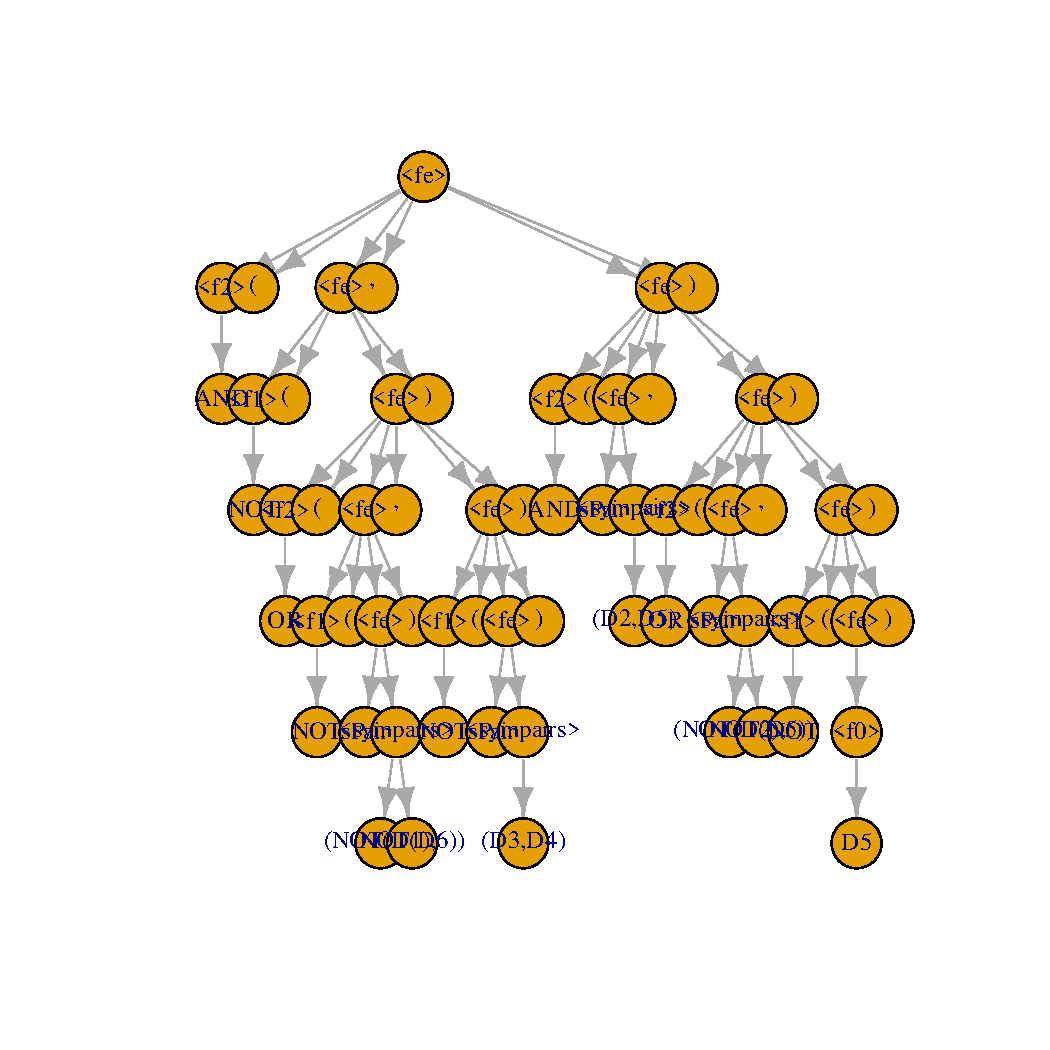
\includegraphics[width=0.5\textwidth, angle=0]
{ExpEDerivationTreeFigure009.pdf}
 \end{center}
 \label{report/ExpEDerivationTreeFigure009.pdf}  
 \end{frame}

% report/ExpEmain137.tex
% ExpE
% Figure: Plot of last xegaRun for Treatment BoolT5sgp6k of Experiment ExpE
% Thu May  8 17:40:55 2025
 \begin{frame}
 \frametitle{ Plot of last xegaRun for Treatment BoolT5sgp6k of Experiment ExpE }
 \begin{center}
\includegraphics[width=0.5\textwidth, angle=-90]
{ExpEPlotPopStatsFigure009.eps}
 \end{center}
 \label{report/ExpEPlotPopStatsFigure009.eps}  
 \end{frame}

% report/ExpEmain138.tex
\miniframeson
\section{C xega}
% report/ExpEmain139.tex
% ExpE
% Table:  All parameters of xegaRun of treatment BoolT4sgp2k 

% Thu May  8 17:40:55 2025
 \begin{frame}
 \fontsize{8pt}{9pt}\selectfont
 \frametitle{  All parameters of xegaRun of treatment BoolT4sgp2k 
 }
% latex table generated in R 4.4.3 by xtable 1.8-4 package
% Wed May 14 17:33:42 2025
\begin{table}[ht]
\centering
\begin{tabular}{rr}
  \hline
 & Parameter Values \\ 
  \hline
penv & 2-Symmetry Problem \\ 
  grammar & /home/dj2333/dev/cran/kSymmetry/BNF/AndOrNotTuned4.txt \\ 
  max & FALSE \\ 
  algorithm & sgp \\ 
  popsize & 200 \\ 
  generations & 500 \\ 
  crossrate & 0.2 \\ 
  mutrate & 0.4 \\ 
  elitist & TRUE \\ 
  replay & 0 \\ 
  maxdepth & 7 \\ 
  maxtrials & 5 \\ 
  codons & 80 \\ 
  codonBits & 0 \\ 
  codonPrecision & LCM \\ 
   \hline
\end{tabular}
\caption{ All parameters of xegaRun of treatment BoolT4sgp2k 
 (Part 1)} 
\end{table}

 \label{ExpEtParmTable040.tex}  
 \end{frame}

 % Label:  \label{ExpEtParmTable040.tex}  
% report/ExpEmain140.tex
% ExpE
% Table:  All parameters of xegaRun of treatment BoolT4sgp2k 

% Thu May  8 17:40:55 2025
 \begin{frame}
 \fontsize{8pt}{9pt}\selectfont
 \frametitle{  All parameters of xegaRun of treatment BoolT4sgp2k 
 }
% latex table generated in R 4.4.3 by xtable 1.8-4 package
% Thu May  8 17:40:55 2025
\begin{table}[ht]
\centering
\begin{tabular}{rr}
  \hline
 & Parameter Values \\ 
  \hline
maxPBias & 0.01 \\ 
  evalmethod & Deterministic \\ 
  evalrep & 1 \\ 
  reportEvalErrors & TRUE \\ 
  genemap & Bin2Dec \\ 
  decoder & DecodeGene \\ 
  crossrate2 & 0.4 \\ 
  ivcrossrate & Const \\ 
  crossover & Cross2Gene \\ 
  uCrossSwap & 0.2 \\ 
  mincrossdepth & 1 \\ 
  maxcrossdepth & 7 \\ 
  ivmutrate & Const \\ 
  mutrate2 & 0.8 \\ 
  bitmutrate & 0.005 \\ 
   \hline
\end{tabular}
\caption{ All parameters of xegaRun of treatment BoolT4sgp2k 
 (Part 2)} 
\end{table}

 \label{ExpEtParmTable041.tex}  
 \end{frame}

 % Label:  \label{ExpEtParmTable041.tex}  
% report/ExpEmain141.tex
% ExpE
% Table:  All parameters of xegaRun of treatment BoolT4sgp2k 

% Thu May  8 17:40:55 2025
 \begin{frame}
 \fontsize{8pt}{9pt}\selectfont
 \frametitle{  All parameters of xegaRun of treatment BoolT4sgp2k 
 }
% latex table generated in R 4.4.3 by xtable 1.8-4 package
% Thu May  8 17:40:55 2025
\begin{table}[ht]
\centering
\begin{tabular}{rr}
  \hline
 & Parameter Values \\ 
  \hline
bitmutrate2 & 0.01 \\ 
  maxmutdepth & 3 \\ 
  minmutinsertiondepth & 1 \\ 
  maxmutinsertiondepth & 7 \\ 
  lambda & 0.05 \\ 
  max2opt & 100 \\ 
  scalefactor1 & 0.9 \\ 
  scalefactor2 & 0.3 \\ 
  scalefactor & Uniform \\ 
  cutoffFit & 0.5 \\ 
  mutation & MutateGene \\ 
  replication & Kid2 \\ 
  initgene & InitGene \\ 
  offset & 1 \\ 
  eps & 0.01 \\ 
   \hline
\end{tabular}
\caption{ All parameters of xegaRun of treatment BoolT4sgp2k 
 (Part 3)} 
\end{table}

 \label{ExpEtParmTable042.tex}  
 \end{frame}

 % Label:  \label{ExpEtParmTable042.tex}  
% report/ExpEmain142.tex
% ExpE
% Table:  All parameters of xegaRun of treatment BoolT4sgp2k 

% Thu May  8 17:40:55 2025
 \begin{frame}
 \fontsize{8pt}{9pt}\selectfont
 \frametitle{  All parameters of xegaRun of treatment BoolT4sgp2k 
 }
% latex table generated in R 4.4.3 by xtable 1.8-4 package
% Thu May  8 17:40:55 2025
\begin{table}[ht]
\centering
\begin{tabular}{rr}
  \hline
 & Parameter Values \\ 
  \hline
tournamentSize & 2 \\ 
  selectionBias & 1.5 \\ 
  maxTSR & 1.5 \\ 
  selection & SUS \\ 
  mateselection & SUS \\ 
  selectionContinuation & TRUE \\ 
  scaling & NoScaling \\ 
  scalingThreshold & 0 \\ 
  scalingExp & 1 \\ 
  scalingExp2 & 1 \\ 
  rdmWeight & 1 \\ 
  drMax & 2 \\ 
  drMin & 0.5 \\ 
  dispersionMeasure & var \\ 
  scalingDelay & 1 \\ 
   \hline
\end{tabular}
\caption{ All parameters of xegaRun of treatment BoolT4sgp2k 
 (Part 4)} 
\end{table}

 \label{ExpEtParmTable043.tex}  
 \end{frame}

 % Label:  \label{ExpEtParmTable043.tex}  
% report/ExpEmain143.tex
% ExpE
% Table:  All parameters of xegaRun of treatment BoolT4sgp2k 

% Thu May  8 17:40:55 2025
 \begin{frame}
 \fontsize{8pt}{9pt}\selectfont
 \frametitle{  All parameters of xegaRun of treatment BoolT4sgp2k 
 }
% latex table generated in R 4.4.3 by xtable 1.8-4 package
% Thu May  8 17:40:55 2025
\begin{table}[ht]
\centering
\begin{tabular}{rr}
  \hline
 & Parameter Values \\ 
  \hline
accept & All \\ 
  alpha & 0.99 \\ 
  beta & 2 \\ 
  cooling & ExponentialMultiplicative \\ 
  coolingPower & 1 \\ 
  temp0 & 40 \\ 
  tempN & 0.01 \\ 
  verbose & 1 \\ 
  logevals & FALSE \\ 
  allsolutions & FALSE \\ 
  early & FALSE \\ 
  terminationCondition & AbsoluteError \\ 
  terminationEps & -0.1 \\ 
  terminationThreshold & 0 \\ 
  worstFitness & -4 \\ 
   \hline
\end{tabular}
\caption{ All parameters of xegaRun of treatment BoolT4sgp2k 
 (Part 5)} 
\end{table}

 \label{ExpEtParmTable044.tex}  
 \end{frame}

 % Label:  \label{ExpEtParmTable044.tex}  
% report/ExpEmain144.tex
% ExpE
% Table:  All parameters of xegaRun of treatment BoolT4sgp2k 

% Thu May  8 17:40:55 2025
 \begin{frame}
 \fontsize{8pt}{9pt}\selectfont
 \frametitle{  All parameters of xegaRun of treatment BoolT4sgp2k 
 }
% latex table generated in R 4.4.3 by xtable 1.8-4 package
% Thu May  8 17:40:55 2025
\begin{table}[ht]
\centering
\begin{tabular}{rr}
  \hline
 & Parameter Values \\ 
  \hline
PACdelta & 0.01 \\ 
  fSpace & Hilbert \\ 
  cores & 16 \\ 
  executionModel & MultiCore \\ 
  uParApply & NULL \\ 
  Cluster & NULL \\ 
  profile & FALSE \\ 
  batch & FALSE \\ 
  path & . \\ 
  semantics & byValue \\ 
   \hline
\end{tabular}
\caption{ All parameters of xegaRun of treatment BoolT4sgp2k 
 (Part 6)} 
\end{table}

 \label{ExpEtParmTable045.tex}  
 \end{frame}

 % Label:  \label{ExpEtParmTable045.tex}  
% report/ExpEmain145.tex
\end{document}
